\chapter{程序模拟结果及对实际机器的模拟研究} \label{chap:Simulation}
随着加速器束流流强的增大,为了对束流进行精确的模拟和研究,我们需要模拟的粒子数目增加了几个量级。
在这种趋势下,束流模拟软件的效率至关重要。
第\ref{chap:Code}章介绍了束流模拟程序在GPU和CPU上的并行实现,
在本章中,小节\ref{section:PIC_performance}和\ref{section:Symplectic_performance}将分别对PIC算法和Symplectic算法的GPU并行性能进行了测试。

之后,我们使用束流模拟软件研究了几个空间电荷相关的问题。
首先,第\ref{section:3rd_order_simulation}节介绍了对空间电荷导致的三阶共振进行的模拟研究,
之后,在第\ref{section:ADS_simulation}节我们使用P-TOPO程序对C-ADS的注入器I进行了模拟研究。

\section{PIC算法性能}             \label{section:PIC_performance}

\subsection{单GPU性能提升-GTX1060}
首先,我们通过对比CPU程序和GPU程序的运行速度,来得到GPU程序的的加速比。加速比等于CPU程序耗时除以GPU程序耗时。测试使用的格点数为 64*64*64,图\ref{fig:PIC_speedup_1GPU}和表\ref{tab:PIC_speedup_1GPU}是粒子数从16k到1.6m时CPU程序和GPU程序各部分耗时以及加速比。程序消耗的总时间的加速比大约有40,然而每一部分的加速比有很大不同。

其中,橙色柱行代表求解泊松方程,其加速比大约是64,而且并不随粒子数目的变化而变化。事实上,求解泊松方程的计算量主要和格点数相关,而此次测试中我们都是用同样的格点数,因此其耗时基本不变,之后我们会比较在不同格点数情况下求解泊松方程的加速比变化。
灰色柱行代表推动粒子的加速比,其随着粒子数目增加而变大,在粒子数较大时取得超过了70的加速比。
浅蓝色和深蓝色柱行分别是权重差值和粒子信息输出的加速比,其中GPU的权重差值部分包括了粒子排序运算,而且由于其运算的不规则性,加速比较低;而粒子信息输出部分也包含了束团参数的计算,这部分加速比较低是因为输出带宽的限制。


\begin{figure}[!htb]
  \centering
  \begin{tabular}{|l|l|}
    \multicolumn{2}{c}{
    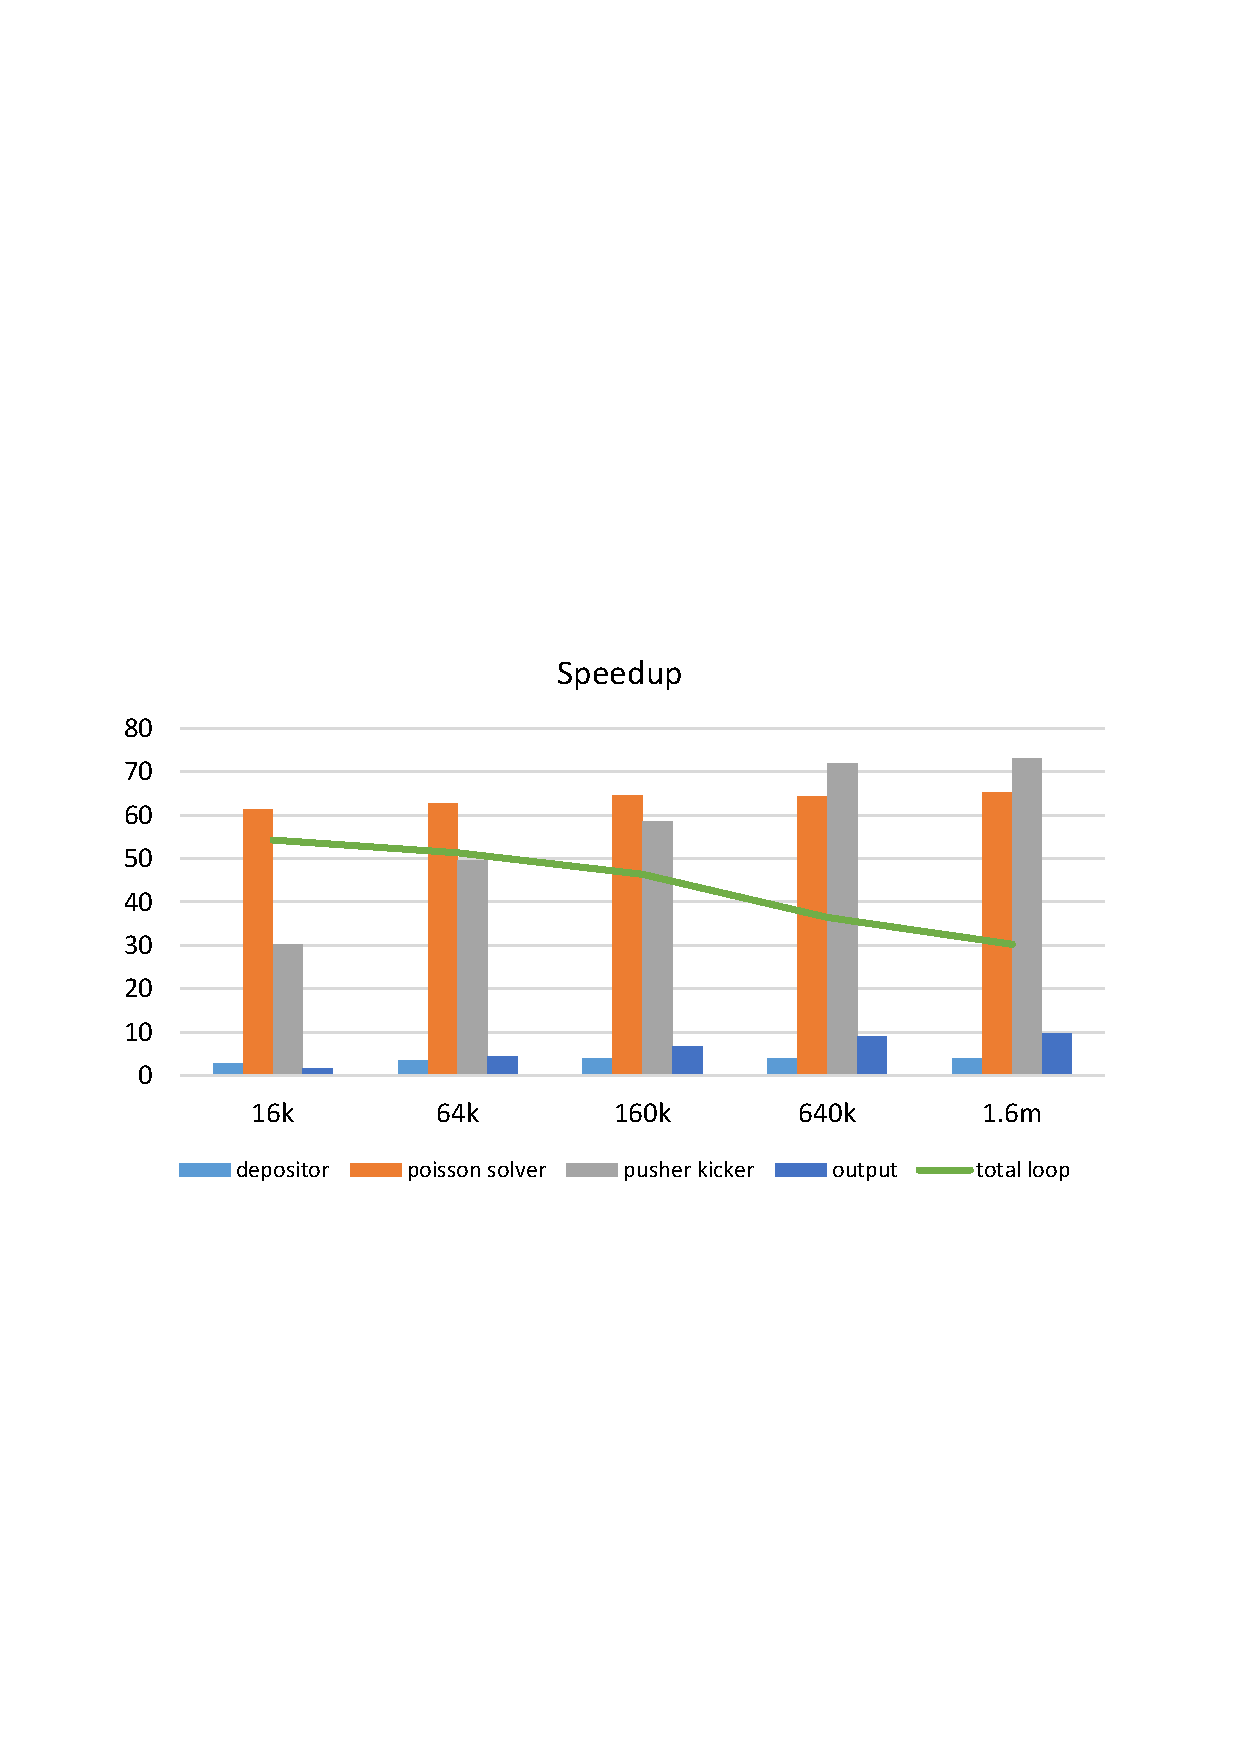
\includegraphics[width=0.9\textwidth]{Img/PIC_speedup_1GPU.pdf}} \\
  \end{tabular}
  \caption{PIC程序在单GPU上的加速比}
  \label{fig:PIC_speedup_1GPU}
\end{figure}

\begin{table}
  \centering
  \begin{tabular}{|l|r|r|r|}
    \hline
    16k                      &    CPU(s)      &     GPU(s)    &  Speedup    \\
    \hline
    depositor (include sort) &    0.16888     &     0.05874   &  2.875043   \\
    Poisson solver           &    26.13173    &     0.42511   &  61.47051   \\
    pusher kicker            &    0.53748	  &     0.01781	  &  30.17855   \\
    output                   &    0.01977     &     0.01149   &  1.720627   \\
    total loop               &    27.78216    &     0.51199   &  54.26309   \\
    \hline
    64k                      &    CPU(s)      &     GPU(s)    &  Speedup    \\
    \hline
    depositor (include sort) &    0.3897      &     0.10847   &  3.592698   \\
    Poisson solver           &    26.08269    &     0.41554   &  62.76818   \\
    pusher kicker            &    2.00422	  &     0.04032	  &  49.70784   \\
    output                   &    0.0641      &     0.01433   &  4.473133   \\
    total loop               &    29.54123    &     0.57598   &  51.28864   \\
    \hline
    160k                     &    CPU(s)      &     GPU(s)    &  Speedup    \\
    \hline
    depositor (include sort) &    0.82705     &     0.20731   &  3.989436   \\
    Poisson solver           &    25.9208     &     0.40208   &  64.46677   \\
    pusher kicker            &    4.88644	  &     0.08343	  &  58.56934   \\
    output                   &    0.15477     &     0.02316   &  6.682642   \\
    total loop               &    32.94187    &     0.71      &  46.397     \\
    \hline
    640k                     &    CPU(s)      &     GPU(s)    &  Speedup    \\
    \hline
    depositor (include sort) &    2.79413     &     0.71529   &  3.90629    \\
    Poisson solver           &    25.72129    &     0.40045   &  64.23097   \\
    pusher kicker            &    22.48269	  &     0.31207	  &  72.04374   \\
    output                   &    0.62289     &     0.06931   &  8.987015   \\
    total loop               &    53.51193    &     1.46745   &  36.46593   \\
    \hline
    1.6m                     &    CPU(s)      &     GPU(s)    &  Speedup    \\
    \hline
    depositor (include sort) &    6.7528      &     1.73779   &  3.885855   \\
    Poisson solver           &    26.03071    &     0.39894   &  65.24969   \\
    pusher kicker            &    56.05512	  &     0.76562	  &  73.21533   \\
    output                   &    1.56528     &     0.16288   &  9.61002    \\
    total loop               &    90.40391    &     2.99053   &  30.23006   \\
    \hline
  \end{tabular}
  \caption{PIC程序在单GPU上的加速比}
  \label{tab:PIC_speedup_1GPU}
\end{table}

权重差值和粒子信息输出的的加速比较低,从而拉低了整体的加速比。整体的加速比随着粒子数的增加而逐渐变小,其原因是当粒子数目较小时的时候,求解泊松方程所占得比重较大,从而整体加速比较大;而当粒子数目变大的时候,权重差值所占的时间比重变大,因而整体加速比随之变小。程序各部分耗时在不同粒子数所占比重如图\ref{PIC_speedup_1GPU_percentage}所示。

\begin{figure}[!htb]
    \centering
    \begin{subfigure}[b]{0.75\textwidth}
        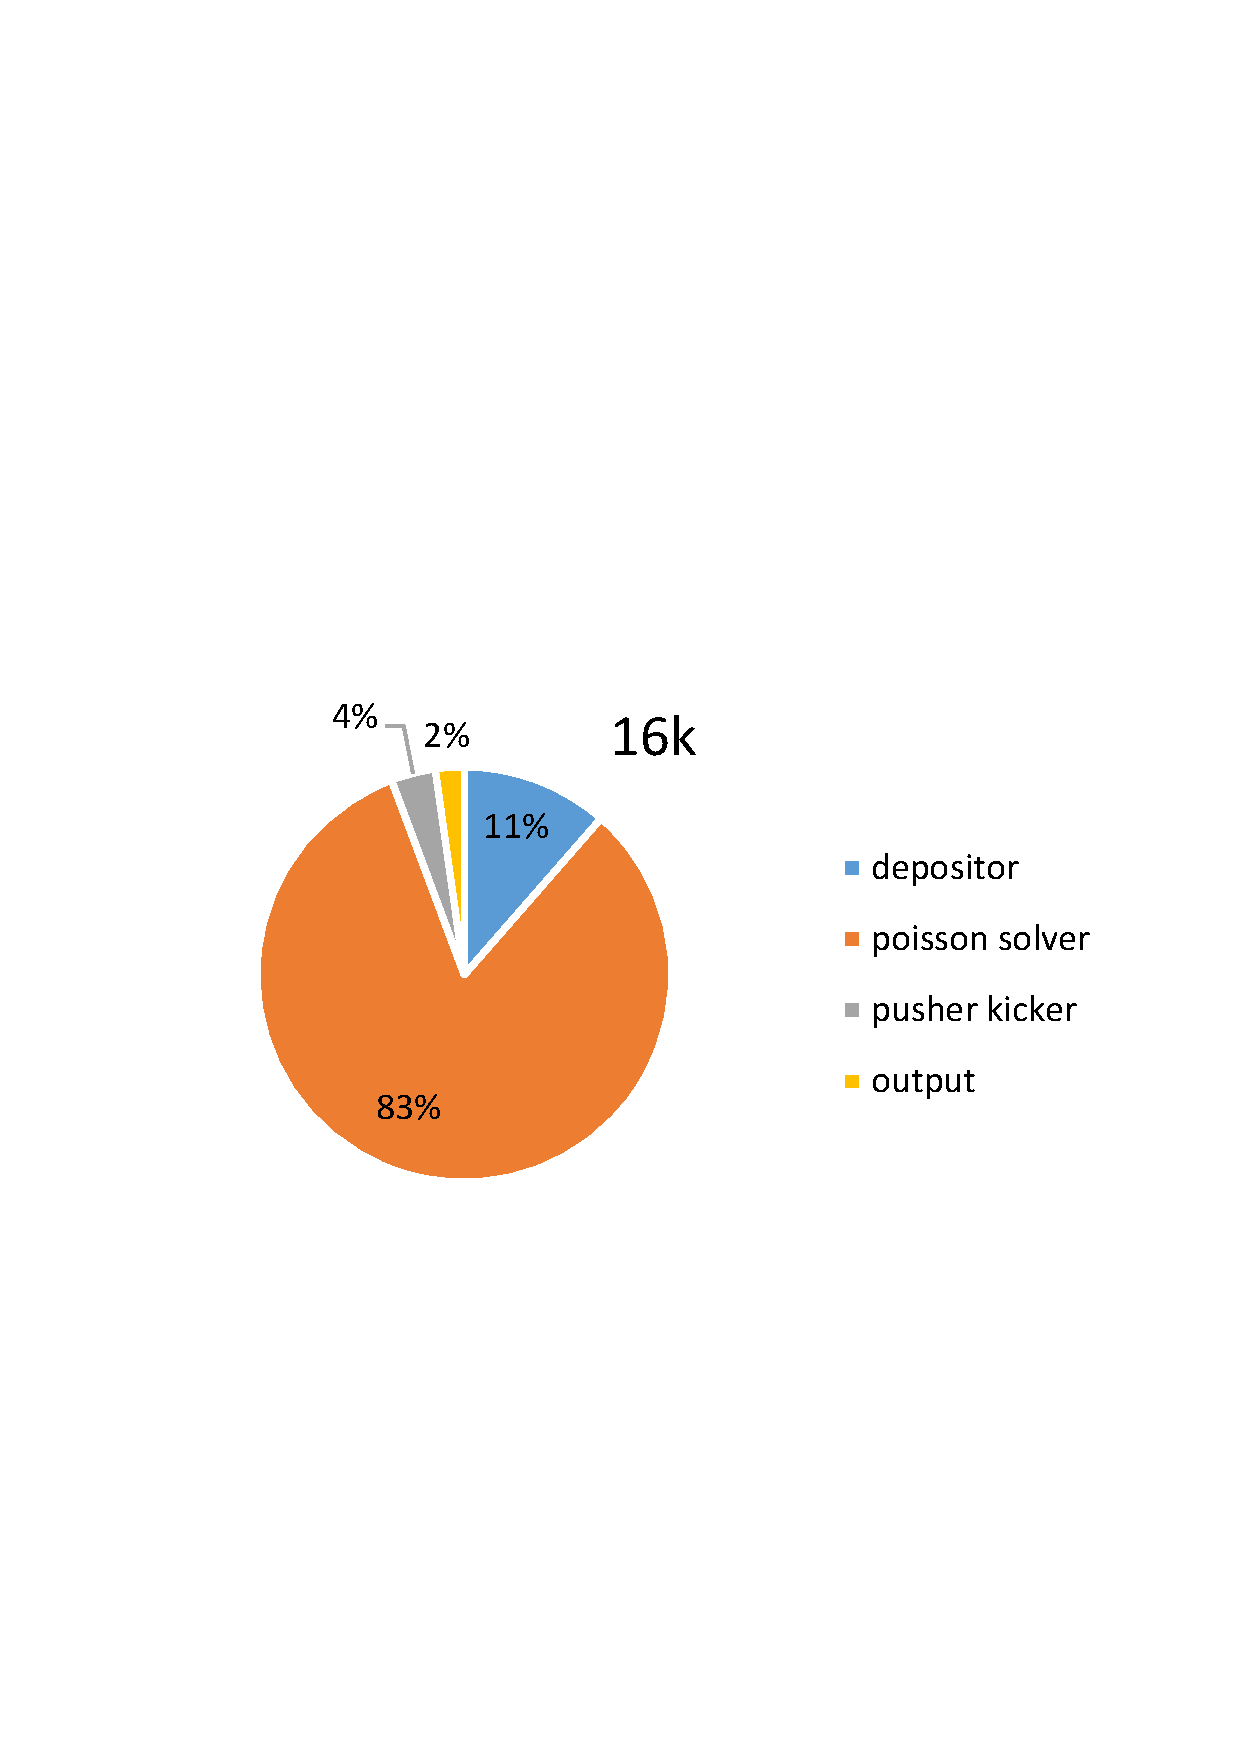
\includegraphics[width=\textwidth]{Img/PIC_speedup_1GPU_percentage1.pdf}
        %\caption{}
    \end{subfigure}
    \quad
    \begin{subfigure}[b]{0.75\textwidth}
        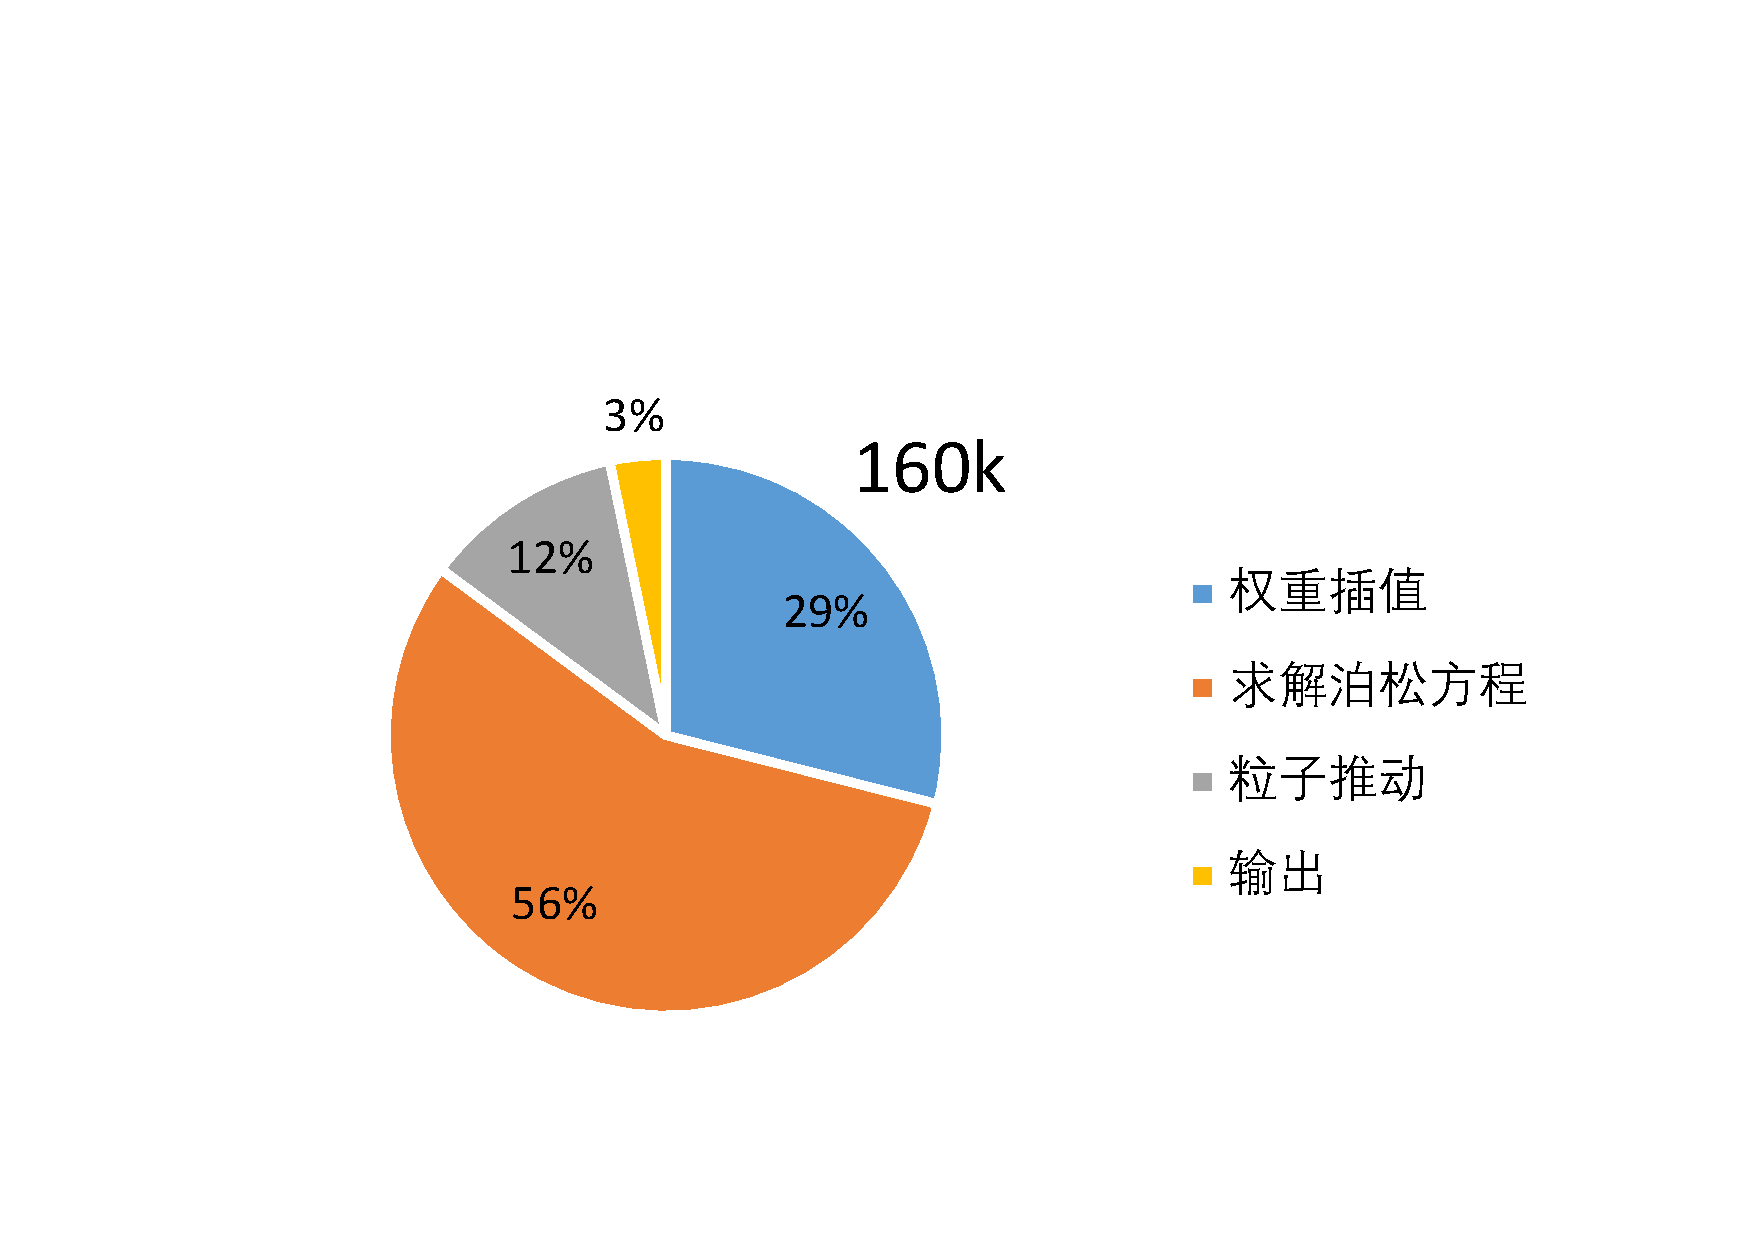
\includegraphics[width=\textwidth]{Img/PIC_speedup_1GPU_percentage2.pdf}
        %\caption{}
    \end{subfigure}
    \quad
    \begin{subfigure}[b]{0.75\textwidth}
        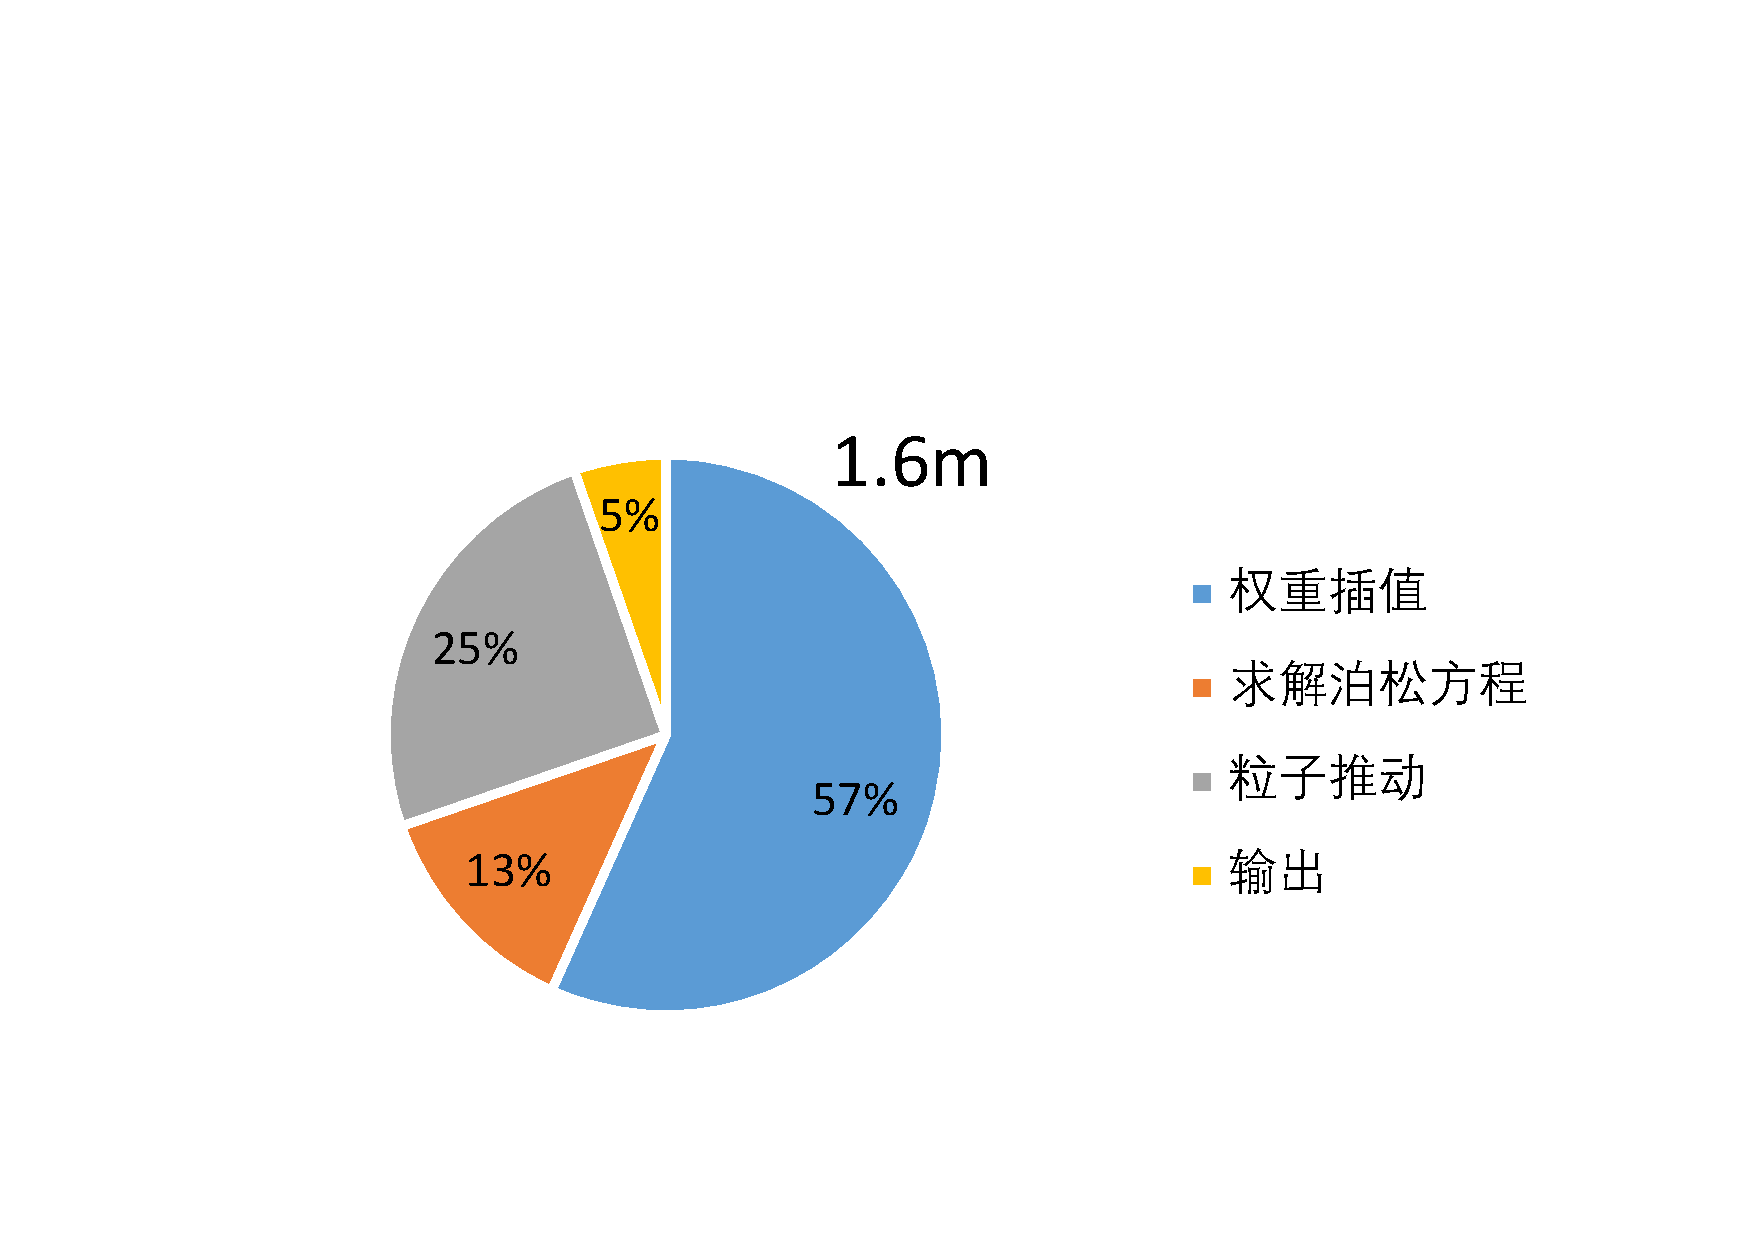
\includegraphics[width=\textwidth]{Img/PIC_speedup_1GPU_percentage3.pdf}
        %\caption{}
    \end{subfigure}
    \caption{程序各部分耗时在不同粒子数时所占百分比}\label{fig:PIC_speedup_1GPU_percentage}
\end{figure}

在上述测试中使用的都是64*64*64个格点数,因此求解泊松方程的时间和加速比都基本不变。在不同的格点数情况下,求解泊松方程的加速比如图\ref{fig:PIC_speedup_1GPU_Poisson}所示。可以看出,求解泊松方程的加速比随着格点数的增加逐渐变大,最终达到了接近70,这是因为格点数越大,其计算量越多,GPU上的负载能够分布得更均匀。在实际模拟中常用的64*64*64个格点和128*128*128个格点中,我们都取得了令人满意的加速比。

\begin{figure}[!htb]
  \centering
  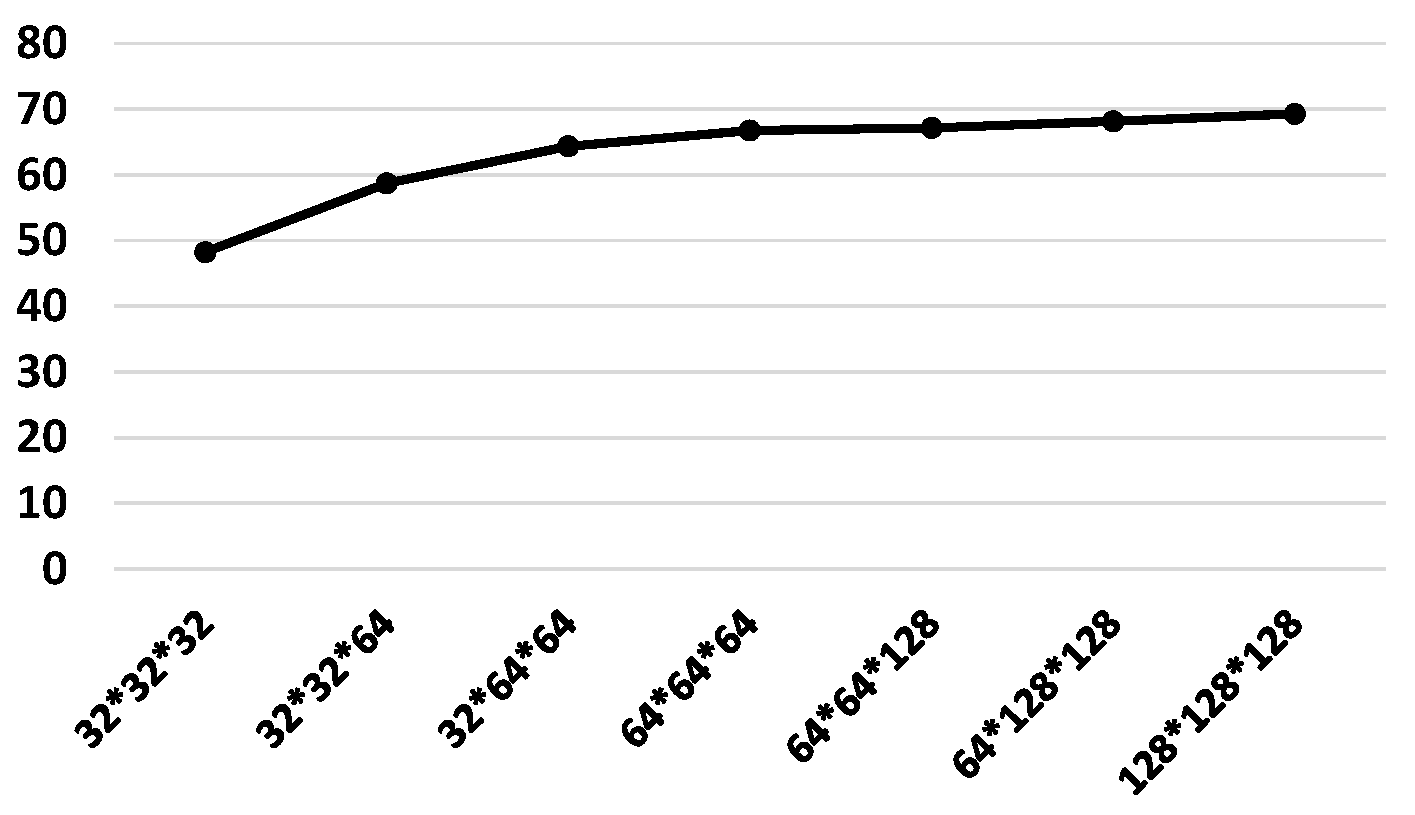
\includegraphics[width=0.9\textwidth]{Img/PIC_speedup_1GPU_Poisson.pdf}
  \caption{不同的格点数情况下单GPU求解泊松方程的加速比}
  \label{fig:PIC_speedup_1GPU_Poisson}
\end{figure}

总之,在单GPU上,程序总体的加速比达到了40,而求解泊松方程的加速比超过到了60,。在一个普通的家用机GPU上运行的速度是在64核机器上运行的两倍。
另外,如小节\ref{section:PIC_GPU_reorder}所述,因为GPU内存大小一般是固定的,而不像CPU内存那样较容易的扩展,所以单GPU的粒子数目存在某个上限,当超过最大粒子数时,应该使用多GPU来进行计算。在接下来的一节中,我们将讨论PIC程序在多GPU上的效率。

\subsection{多GPU性能提升-泰坦}
泰坦(Titan)使用CPU和GPU混合架构,是目前世界上最快,规模最大的计算机集群之一。泰坦的每个节点拥有一个AMD Opteron(16核心)的CPU和一个NVIDIA Tesla K20x (2688核心)的GPU。
泰坦中每个节点只有一个GPU,因此只能通过使用多个节点来使用多个GPU。在这种条件下,GPU之间的通讯只能够通过先将数据拷贝到CPU端,再通过CPU端的节点间网络进行通讯。

图\ref{fig:PIC_speedup_Titan_160k_1}为复制模式求解泊松方程时各个部分所花费的时间随GPU个数的变化,可以看出,因为处于复制模式,求解泊松方程的耗时基本保持不变;由于跟多的GPU个数意味着每个GPU上的粒子数随之减小,粒子推动的耗时随着GPU数目的增加而减少;而由于通讯成本随着GPU数目增加而增加,信息统计和输出耗时也随之增加。各个部分对于GPU的数目并不相同,总体来看,总耗时基本保持不变。

\begin{figure}[!htb]
  \centering
  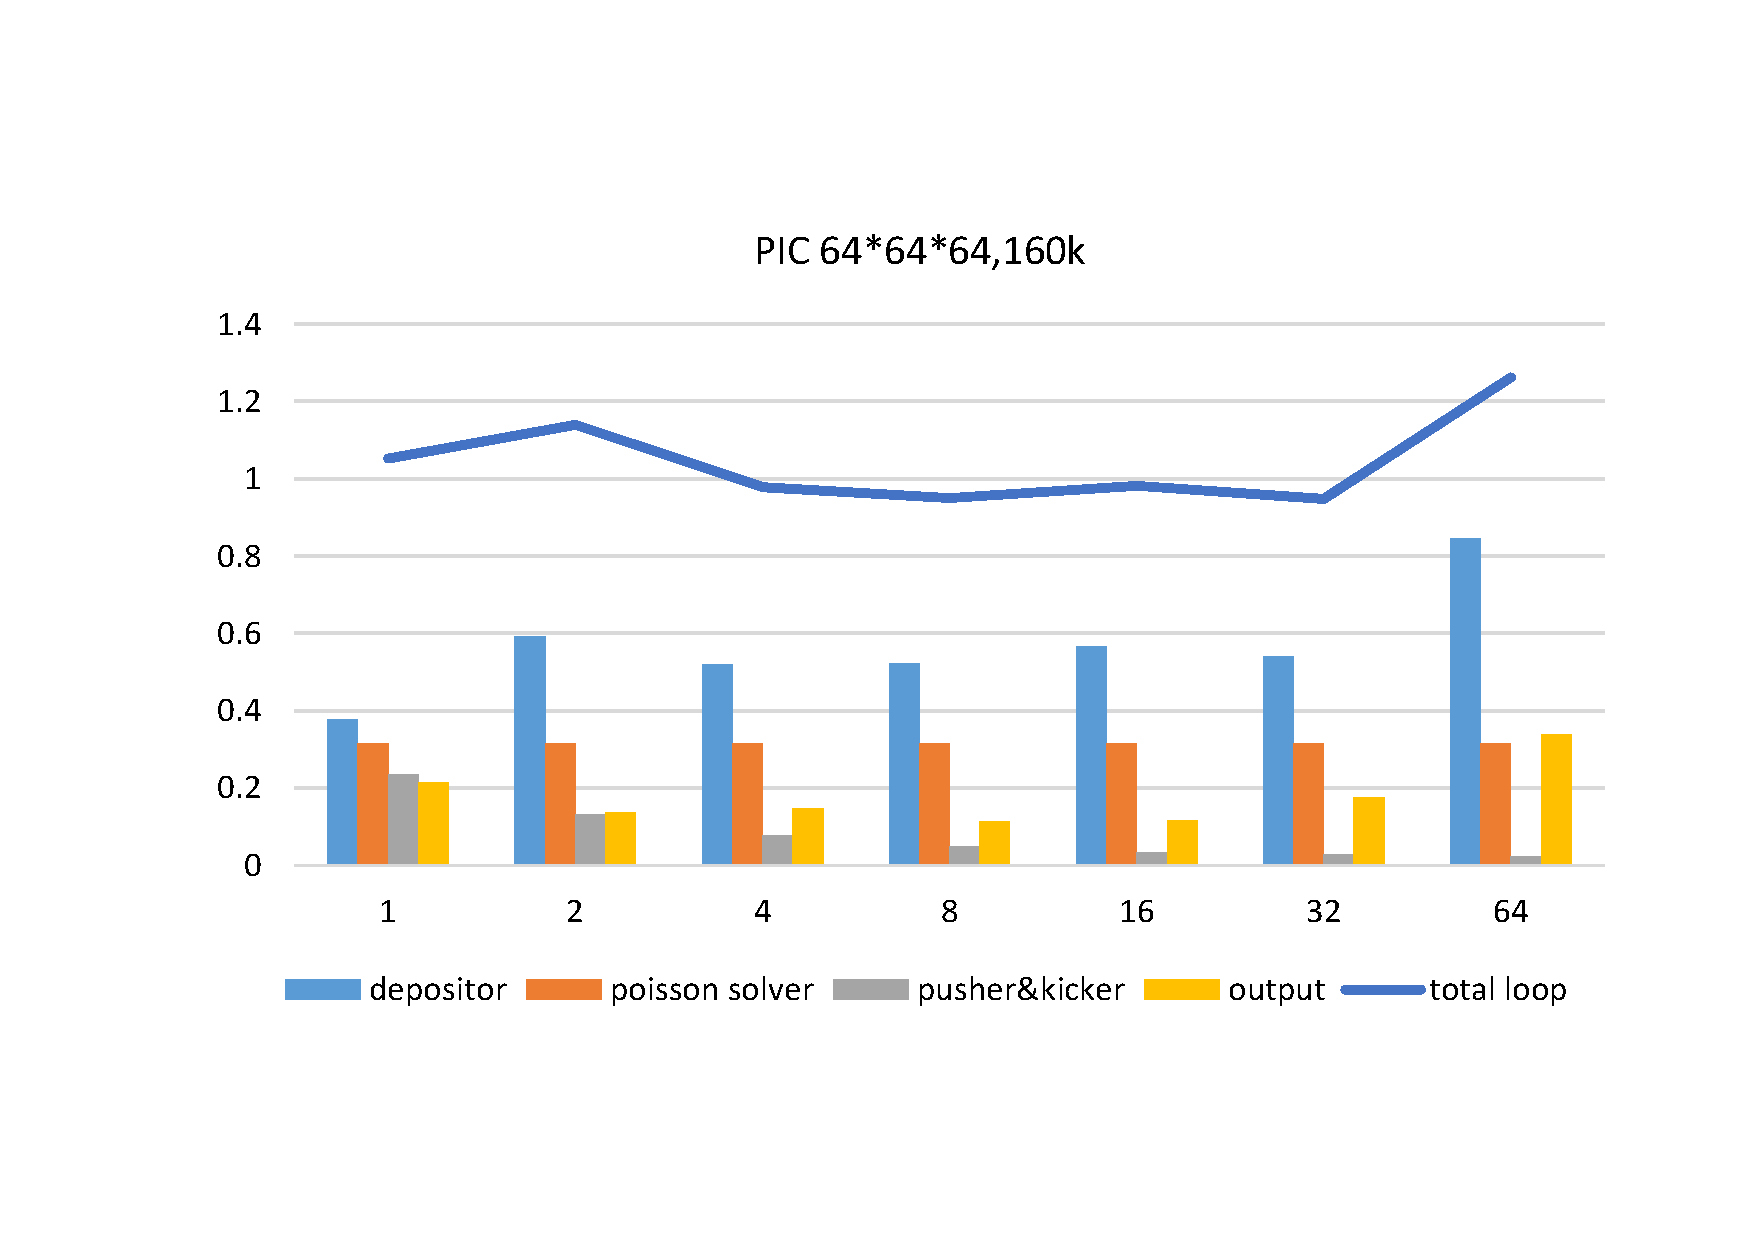
\includegraphics[width=0.9\textwidth]{Img/PIC_speedup_Titan_160k_1.pdf}
  \caption{64*64*64个格点,160k个粒子时,复制模式程序耗时随GPU个数的变化}
  \label{fig:PIC_speedup_Titan_160k_1}
\end{figure}

图\ref{fig:PIC_speedup_Titan_160k_2}和图\ref{fig:PIC_speedup_Titan_160k_1}类似,也是64*64*64各个点,160k个粒子下程序总耗时随着~GPU数目的变化。但是在图\ref{fig:PIC_speedup_Titan_160k_2}中,GPU数目大于等于2的时候,求解泊松方程使用域分解模式。其在各种情况下,都相较复制模式耗时更多,主要是拷贝数据花费了大量时间,这个结果和我们在小节\ref{section:PIC_GPU_Poisson}中讨论的相符。因此在之后的测试中,我们都使用复制模式。

\begin{figure}[!htb]
  \centering
  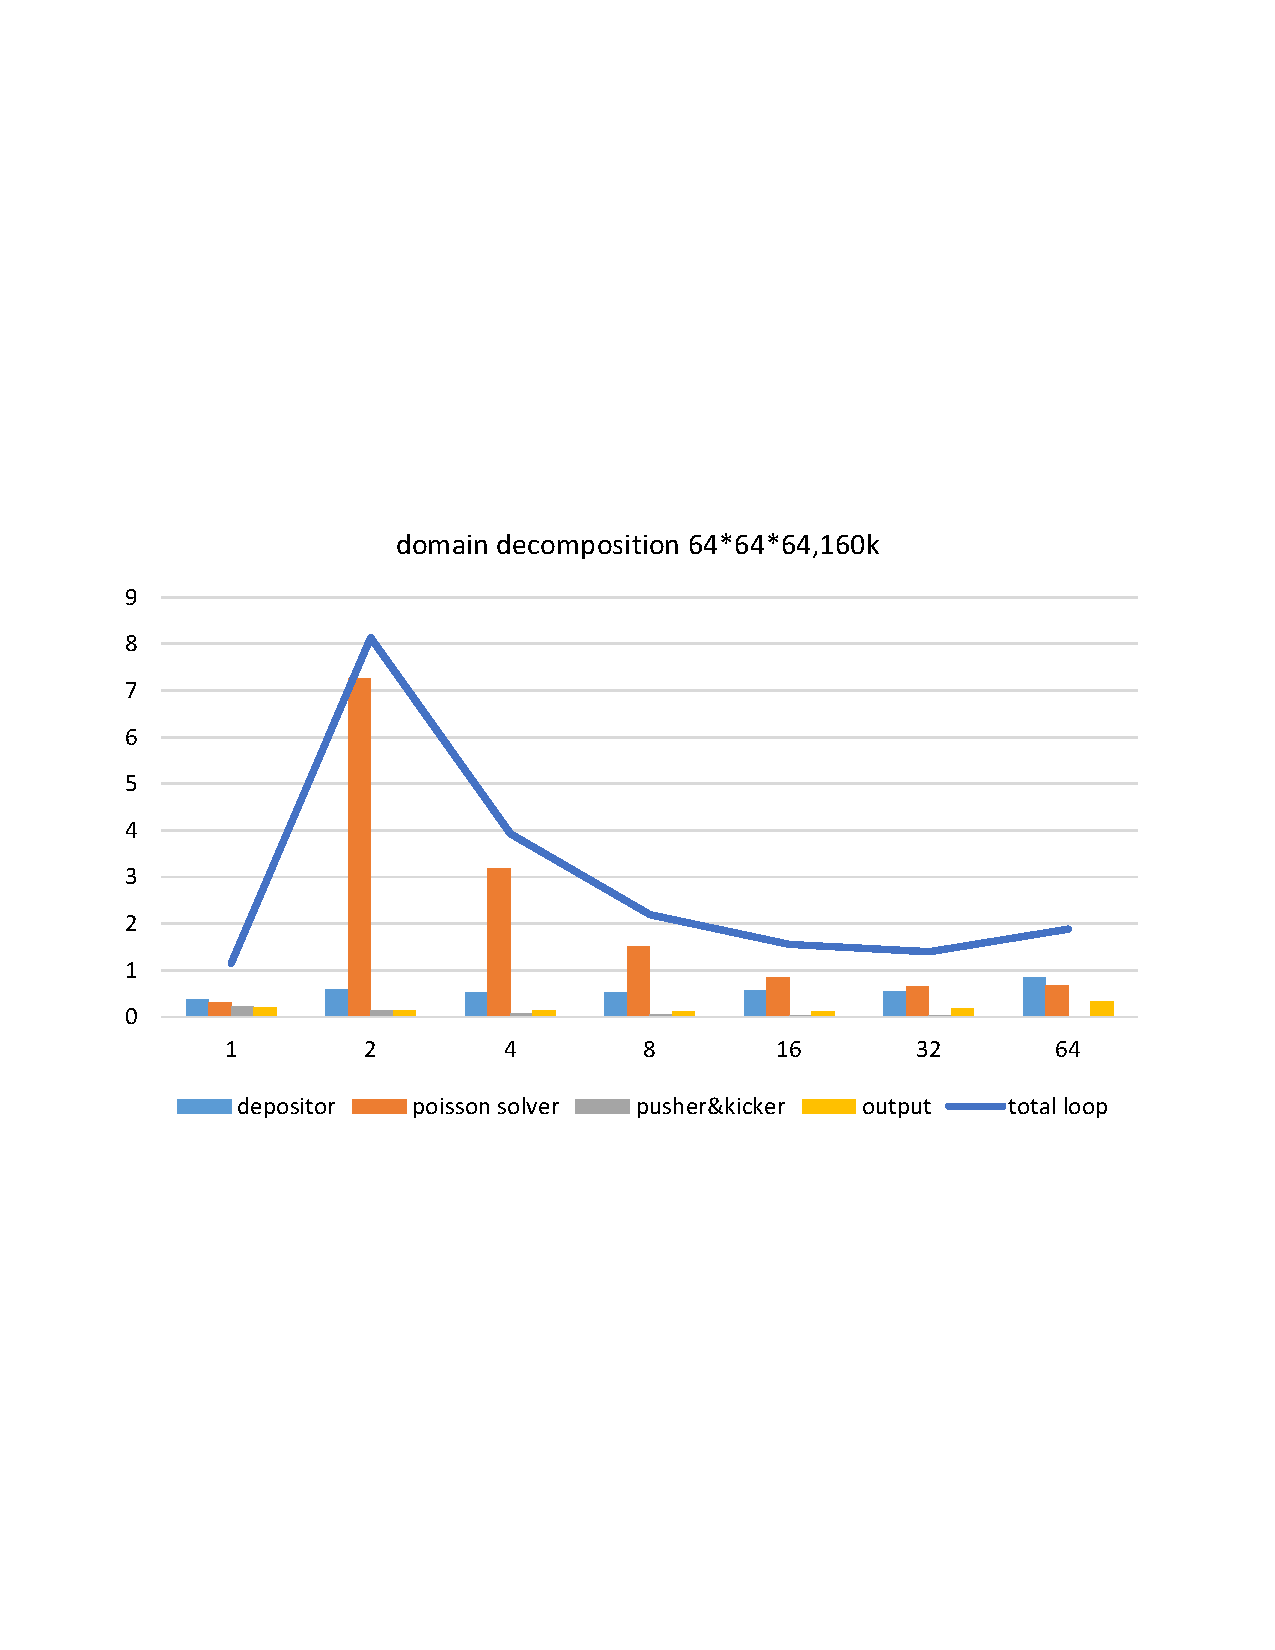
\includegraphics[width=0.9\textwidth]{Img/PIC_speedup_Titan_160k_2.pdf}
  \caption{64*64*64个格点,160k个粒子时,域分解模式程序耗时随GPU个数的变化}
  \label{fig:PIC_speedup_Titan_160k_2}
\end{figure}

当粒子数更大时,耗时的趋势发生了变化。图\ref{fig:PIC_speedup_Titan_1_6m}是粒子数为一百六十万(~1.6m)的结果,粒子数较图\ref{fig:PIC_speedup_Titan_160k_1}变大了十倍。在使用1.6m个粒子时,总耗时随着使用的~GPU数目增加而明显下降,并在32个GPU处到达最小值。
这是因为在大粒子数目情况下,推动粒子和权重差值所占用的时间占了总时间的绝大部分。而由于使用多GPU带来的每个GPU上的粒子数目变少,推动粒子和权重差值能够很好的被多GPU加速。

\begin{figure}[!htb]
  \centering
  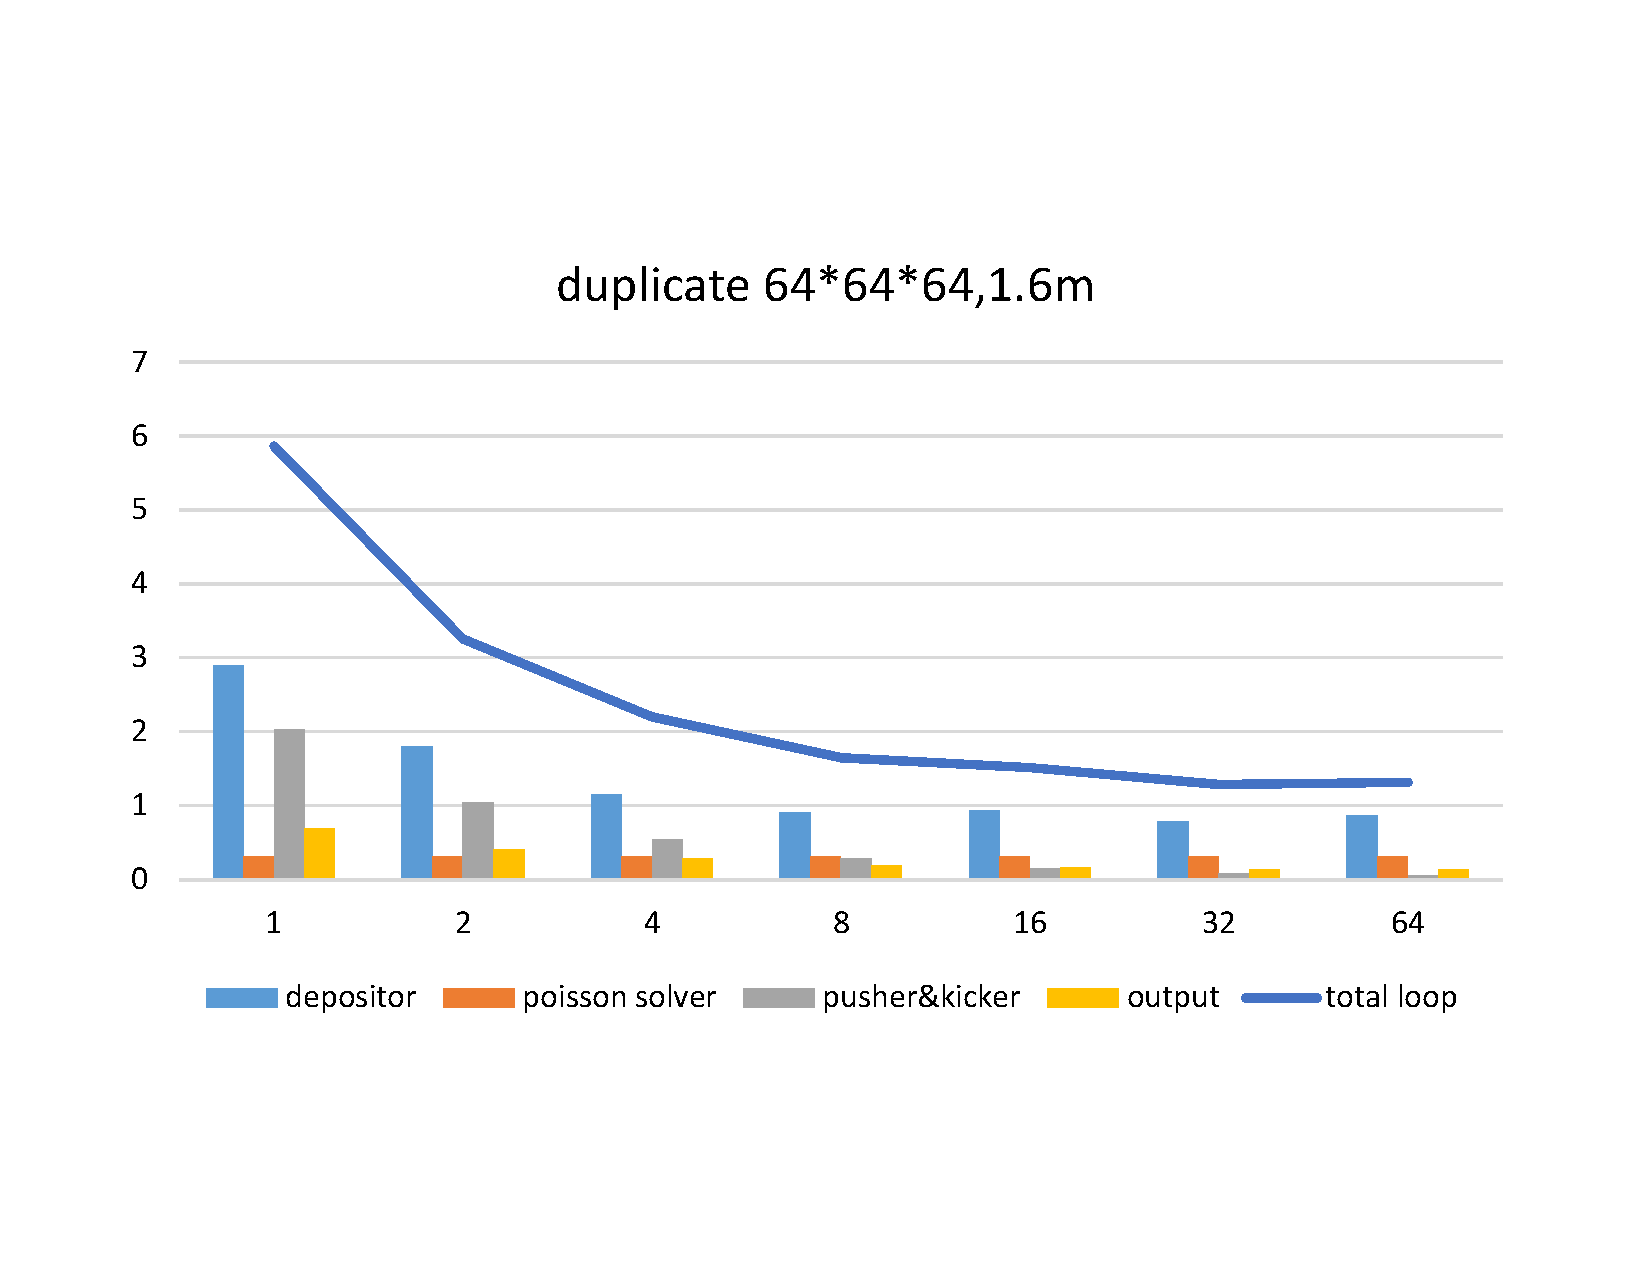
\includegraphics[width=0.9\textwidth]{Img/PIC_speedup_Titan_1_6m.pdf}
  \caption{64*64*64个格点,1.6m个粒子时,程序耗时随GPU个数的变化}
  \label{fig:PIC_speedup_Titan_1_6m}
\end{figure}

我们尝试使用更大的粒子数,一千六百万个粒子(16m),更十倍于前,如图\ref{fig:PIC_speedup_Titan_16m}所示。由于GPU内存大小的限制,程序在这个粒子数下不能仅仅使用1或2个~GPU运行,因此在图\ref{fig:PIC_speedup_Titan_16m}中,GPU数目等于1和等于2的时候没有数据。

超级计算机Titan上使用的GPU型号为NVIDIA K20x,每个GPU有5GB的内存。理想情况下,一个5GB内存能够使用的最大粒子数为六千万(60m)。但这个粒子数是在空间均匀分布下才能使用,而实际上,我们很难达到这个粒子数。一个实际的加速器模拟中我们通常使用KV,WaterBag,或者高斯分布,因此其可用的粒子数目远小于理想数目。

\begin{figure}[!htb]
  \centering
  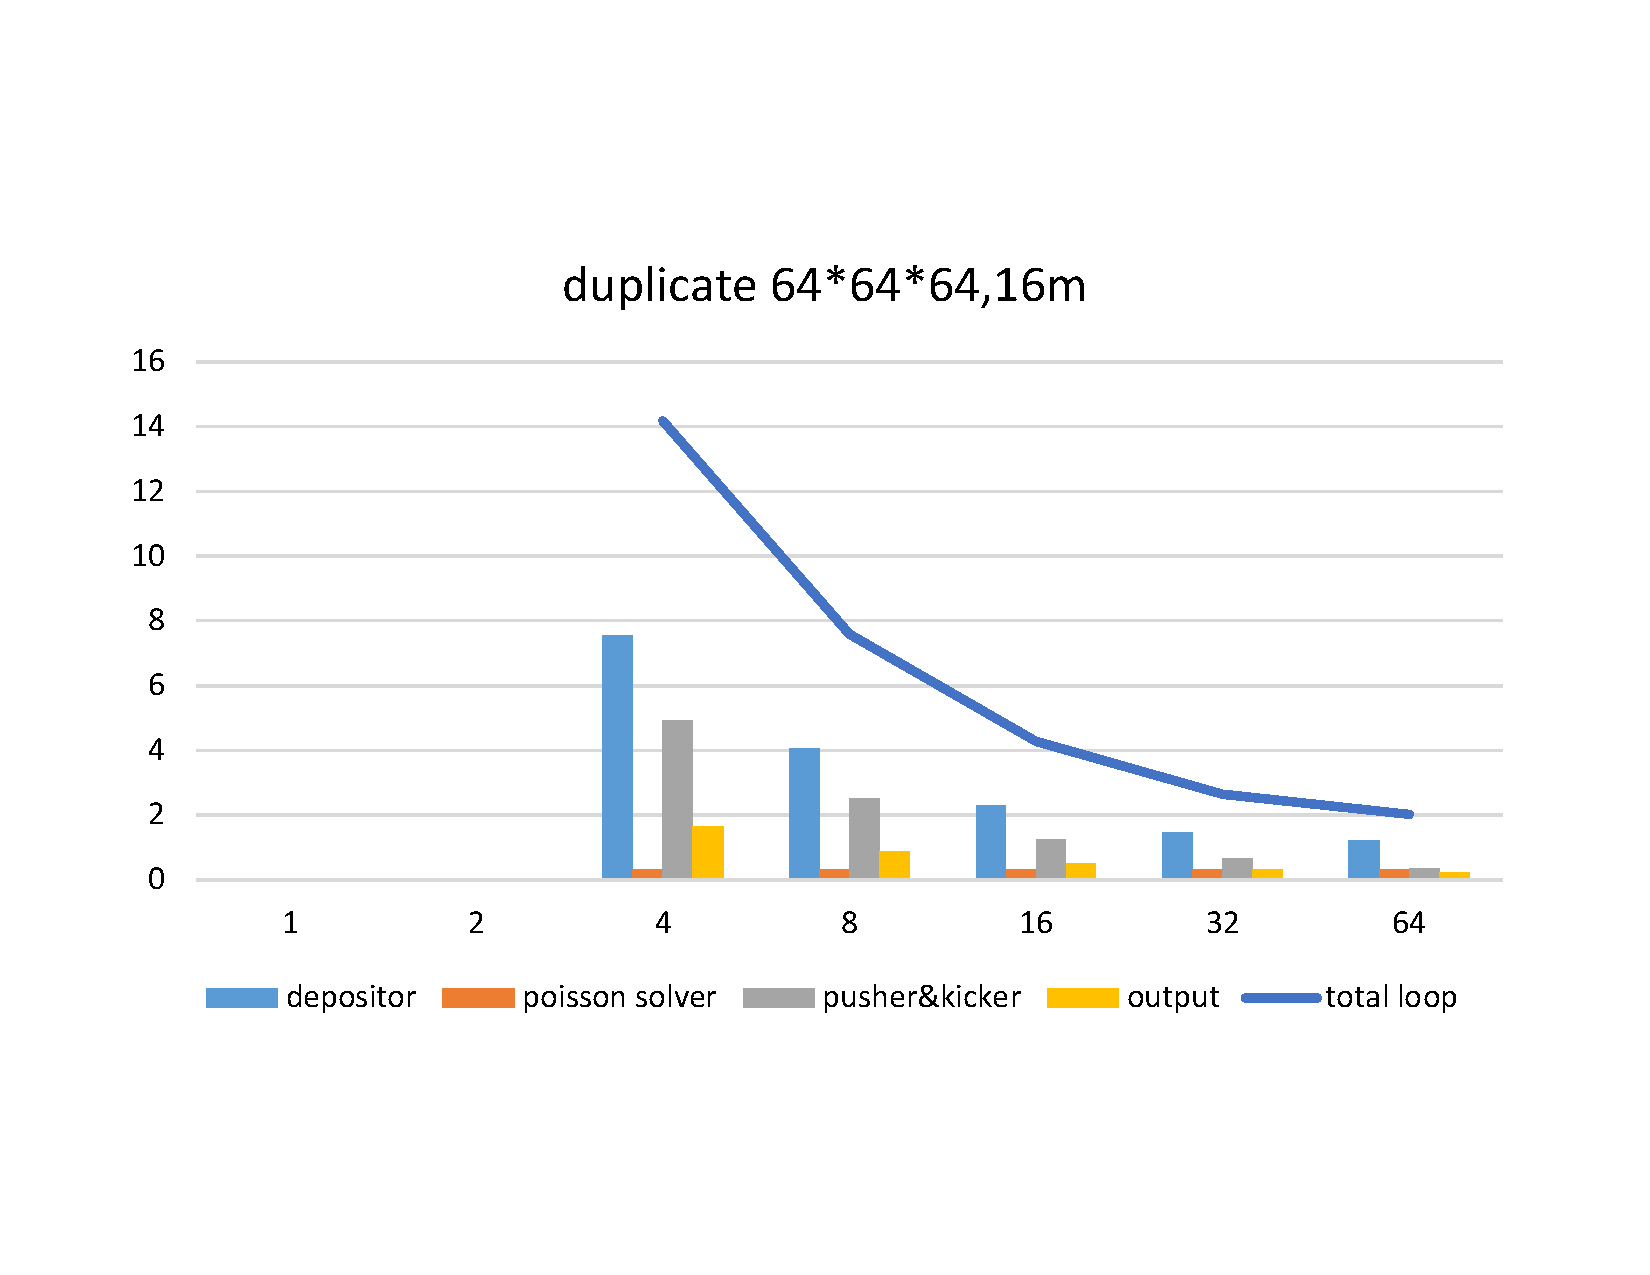
\includegraphics[width=0.9\textwidth]{Img/PIC_speedup_Titan_16m.pdf}
  \caption{64*64*64个格点,16m个粒子时,程序耗时随GPU个数的变化}
  \label{fig:PIC_speedup_Titan_16m}
\end{figure}

\section{Symplectic算法性能}      \label{section:Symplectic_performance}
我们使用GPU程序的性能和可拓展性进行了两个测试,第一个测试使用一个普通的家用GPU:GTX 1060 6GB,测试的结果与在CPU串行运行的程序进行比较。第二个测试使用美国能源部下属的橡树岭国家实验室(ORNL)的GPU集群泰坦,用于测试程序的可扩展性,即程序在多GPU下的表现。

\subsection{单GPU性能提升-GTX1060}
首先,我们将GPU代码的性能与CPU代码进行比较。GPU代码使用GeForce GTX 1060 6GB(Pascal架构)进行测试,而作为对比的CPU代码使用AMD Opteron(tm)6134的一个核心运行,测试的软件环境为Ubuntu 16.04,使用CUDA 8.0版。

加速比由CPU版本运行的运行时间,除以GPU版本的运行时间得到。在本次测试中,我们对空间电荷求解器和整个程序分别进行了比较。空间电荷求解器包括将数据从CPU侧复制到GPU侧,计算空间电荷效应,推动粒子,并将数据复制回CPU侧,而整个程序则包括了除了空间电荷求解器之外的所有其他部分,比如外场推动,输入,统计,输出等等。

从CPU代码简单的移植到GPU代码就可以实现大约200倍的加速,但是我们通过优化可以获得更大的加速比。
在采用了小节\ref{section:symplectic_GPU}中的优化策略后,程序能够充分利用GPU,取得了超过400的加速比。
接下来,如图\ref{fig:OneGPU}所示,我们会讨论分别讨论空间电荷效应和整个程序在不同的问题规模大小下的加速比。

\begin{figure}[!htb]
    \centering
    \begin{subfigure}[b]{0.9\textwidth}
        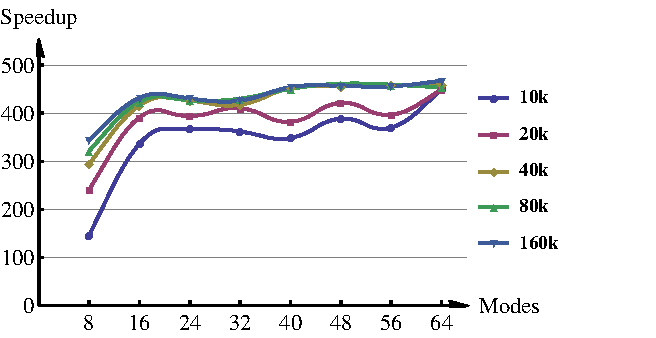
\includegraphics[width=\textwidth]{SymplecticSpaceChargeGPU_AMD13th.pdf}
        \caption{空间电荷效应求解器加速比}
        \label{fig:SCOpt}
    \end{subfigure}
    \quad
    ~ %add desired spacing between images, e. g. ~, \quad, \qquad, \hfill etc.
      %(or a blank line to force the subfigure onto a new line)
    \begin{subfigure}[b]{0.9\textwidth}
        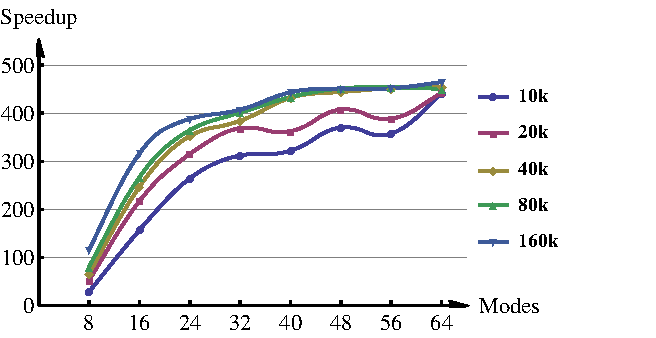
\includegraphics[width=\textwidth]{SymplecticTotalGPU_AMD13th.pdf}
        \caption{程序整体加速比}
        \label{fig:TotalOpt}
    \end{subfigure}
    \caption{单GPU加速比}\label{fig:OneGPU}
\end{figure}

图\ref{fig:SCOpt}为优化后的空间电荷效应求解器的加速比在不同的问题规模下的变化。其中,横坐标为展开的阶数,而纵坐标是加速比,不同的线是不同粒子数目的结果。可以看到,阶数越大加速比越高,这与我们的预期符合,因为阶数越大意味着空间电荷求解器占用的时间在总时间中的比例越大。其中,在$8*8*8$阶时加速比很低,因为在这种模式下的计算量很低。随着阶数的增加,计算量也随之增加,GPU的负载更为平衡,因此取得了更大的加速比。另一方面,粒子数目对于加速比的影响很小,在大阶数的情况下尤为如此。这是因为粒子数目本身远远超出了一个GPU的核心数目(在GTX 1060 上为1280个核心),即时在最低粒子数(10000个粒子)的情况,程序也能有效的使用所有的核心,而随着粒子数目的轻微提升是因为GPU能够在更大运算量的情况下更好的协调和平衡计算资源。

图\ref{fig:TotalOpt}为程序整体的运行时间的加速比,除了空间电荷效应求解之外,程序总体运行时间还包括外部传输矩阵,从Z坐标到T坐标的变换,粒子信息统计以及输入输出。
同空间电荷效应求解器相比,整体时间的加速比在各个问题规模下都略有下降,但是加速比变化的趋势却保持一致。
其中,在低阶情况下,比如$8\times8\times8$阶或$16\times16\times16$阶,因为空间电荷效应求解器所占总时间的比重不大,所以加速比的下降更为严重。
然而,在高阶情况下,空间电荷效应求解所占的时间会占总时间的绝大部分,所以总时间的加速比和空间电荷效应求解的加速比能够基本保持一致。

总之,我们取得了非常好的加速比。对于程序整体的总运行时间,优化的~GPU代码比CPU代码运行速度高450倍;而如果仅仅比较空间电荷效应求解器,其最大加速比超过了460。

\subsection{多GPU性能提升-泰坦}
我们使用超级计算机泰坦进行多GPU测试。
为了测试多GPU的程序可扩展性,我们最多使用了1024个节点进行测试。其中,为了在不同节点的GPU上交换信息,我们需要先把GPU上的数据拷贝到CPU侧,再使用MPI协议在不用节点之间交换数据,最后再将交换后的信息拷贝回GPU侧。
在本次测试中,我们使用16$\times$16$\times$16阶进行测试,使用这个阶数是为了精确度和计算速度之间的平衡,也是我们在实际模拟中最常用的阶数。
如图\ref{fig:Titan}所示,我们分别讨论了空间电荷效应和整个程序在不同的粒子数目下,在不同的节点数上的加速比。其中,横轴为节点数目,纵周围加速比,加速比有多节点的运行时间除以单节点的运行时间得到,不同线是不同粒子数目的结果。

\begin{figure}[!htb]
    \centering
    \begin{subfigure}[b]{0.9\textwidth}
        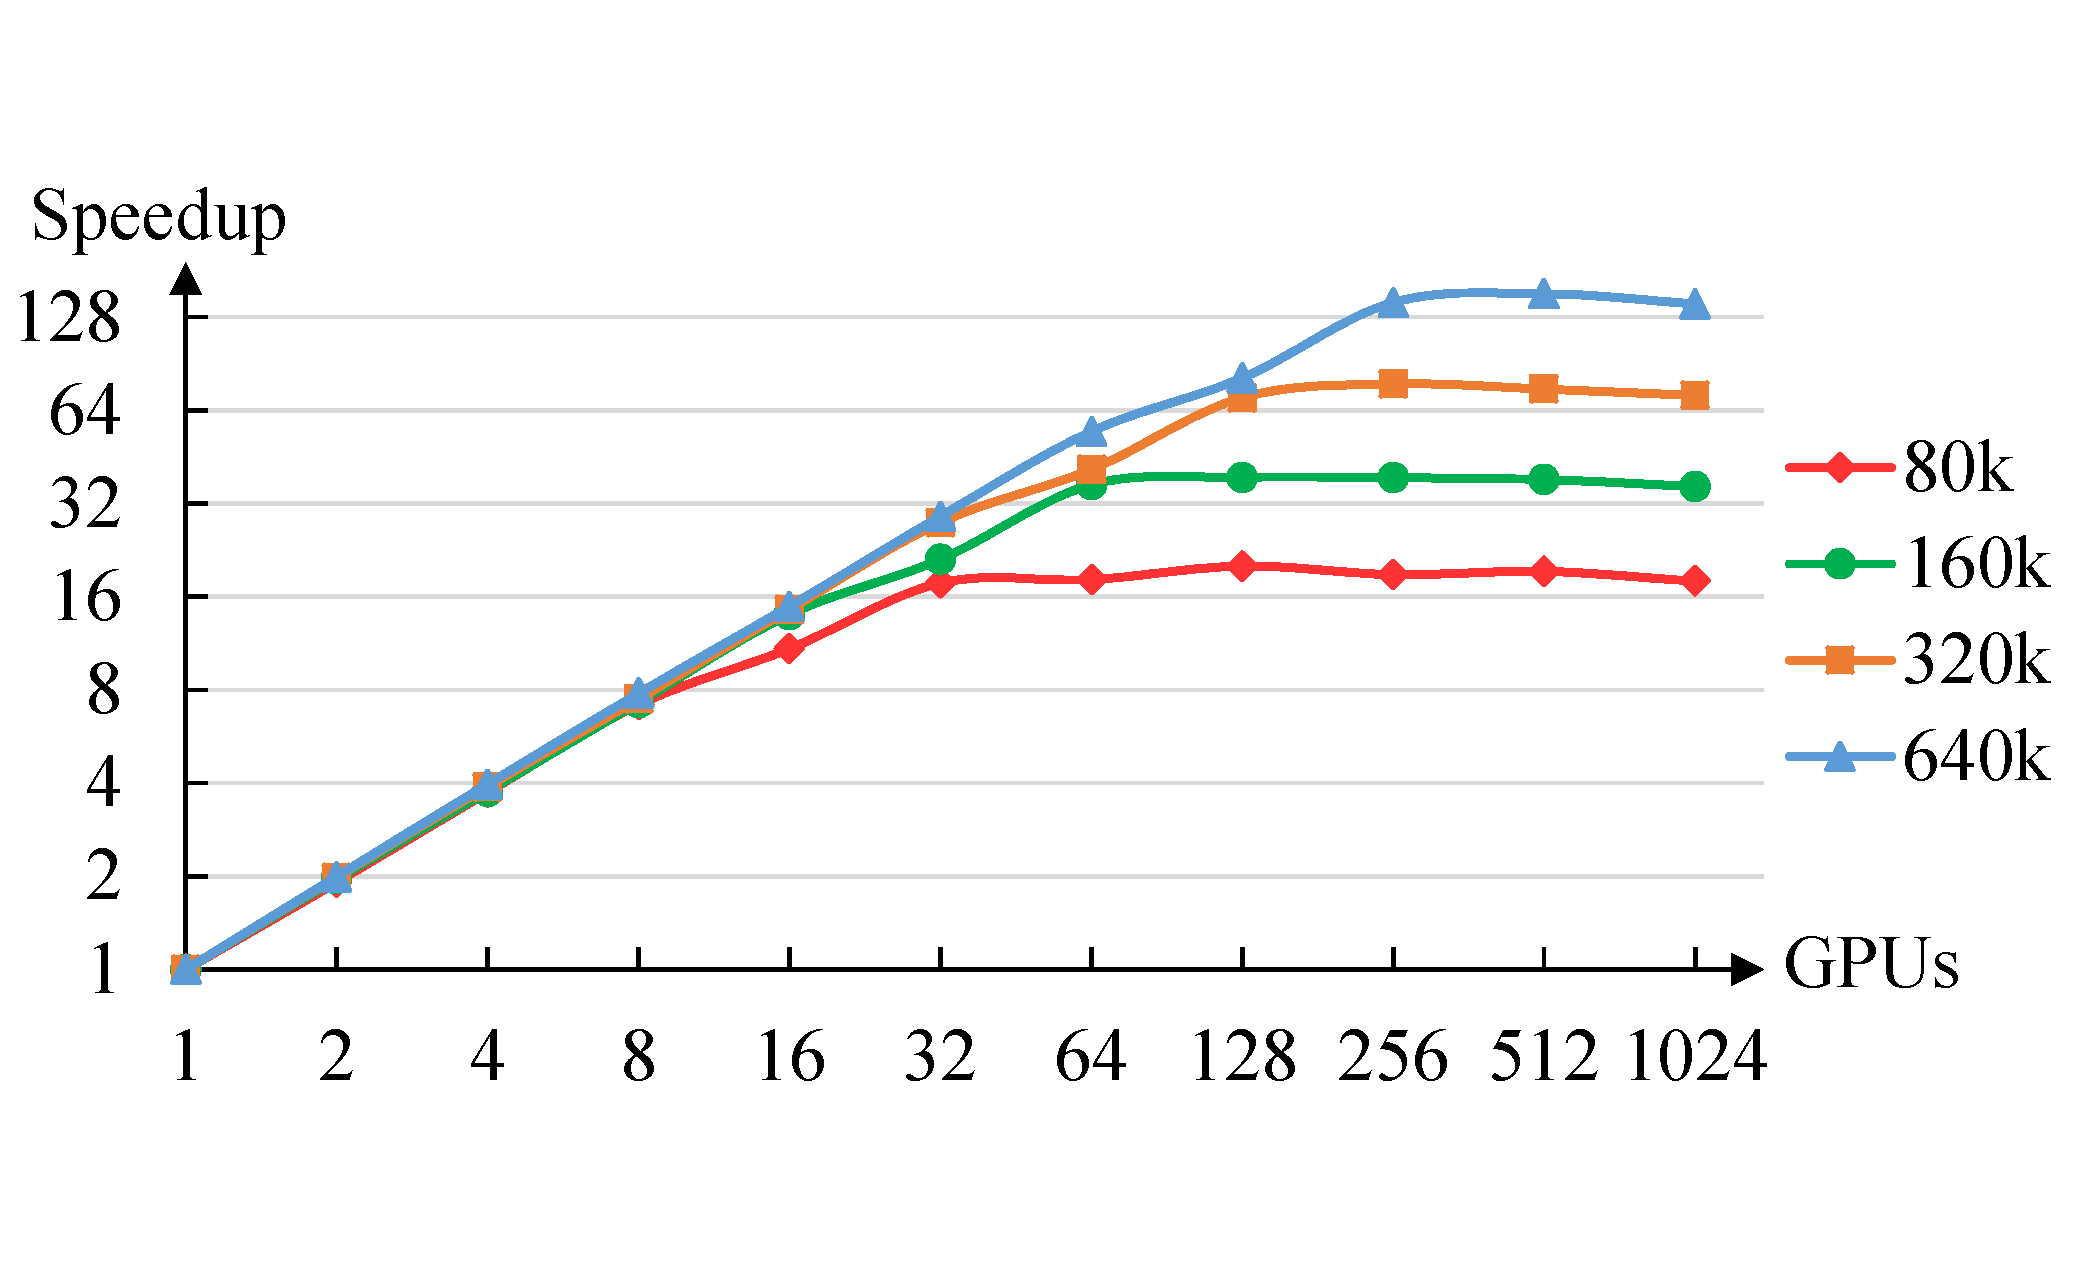
\includegraphics[width=\textwidth]{Img/640k_speedup_of_space_charge_kicker5log.pdf}
        \caption{空间电荷效应求解器加速比}
        \label{fig:SCTitan}
    \end{subfigure}
    \quad
    ~ %add desired spacing between images, e. g. ~, \quad, \qquad, \hfill etc.
      %(or a blank line to force the subfigure onto a new line)
    \begin{subfigure}[b]{0.9\textwidth}
        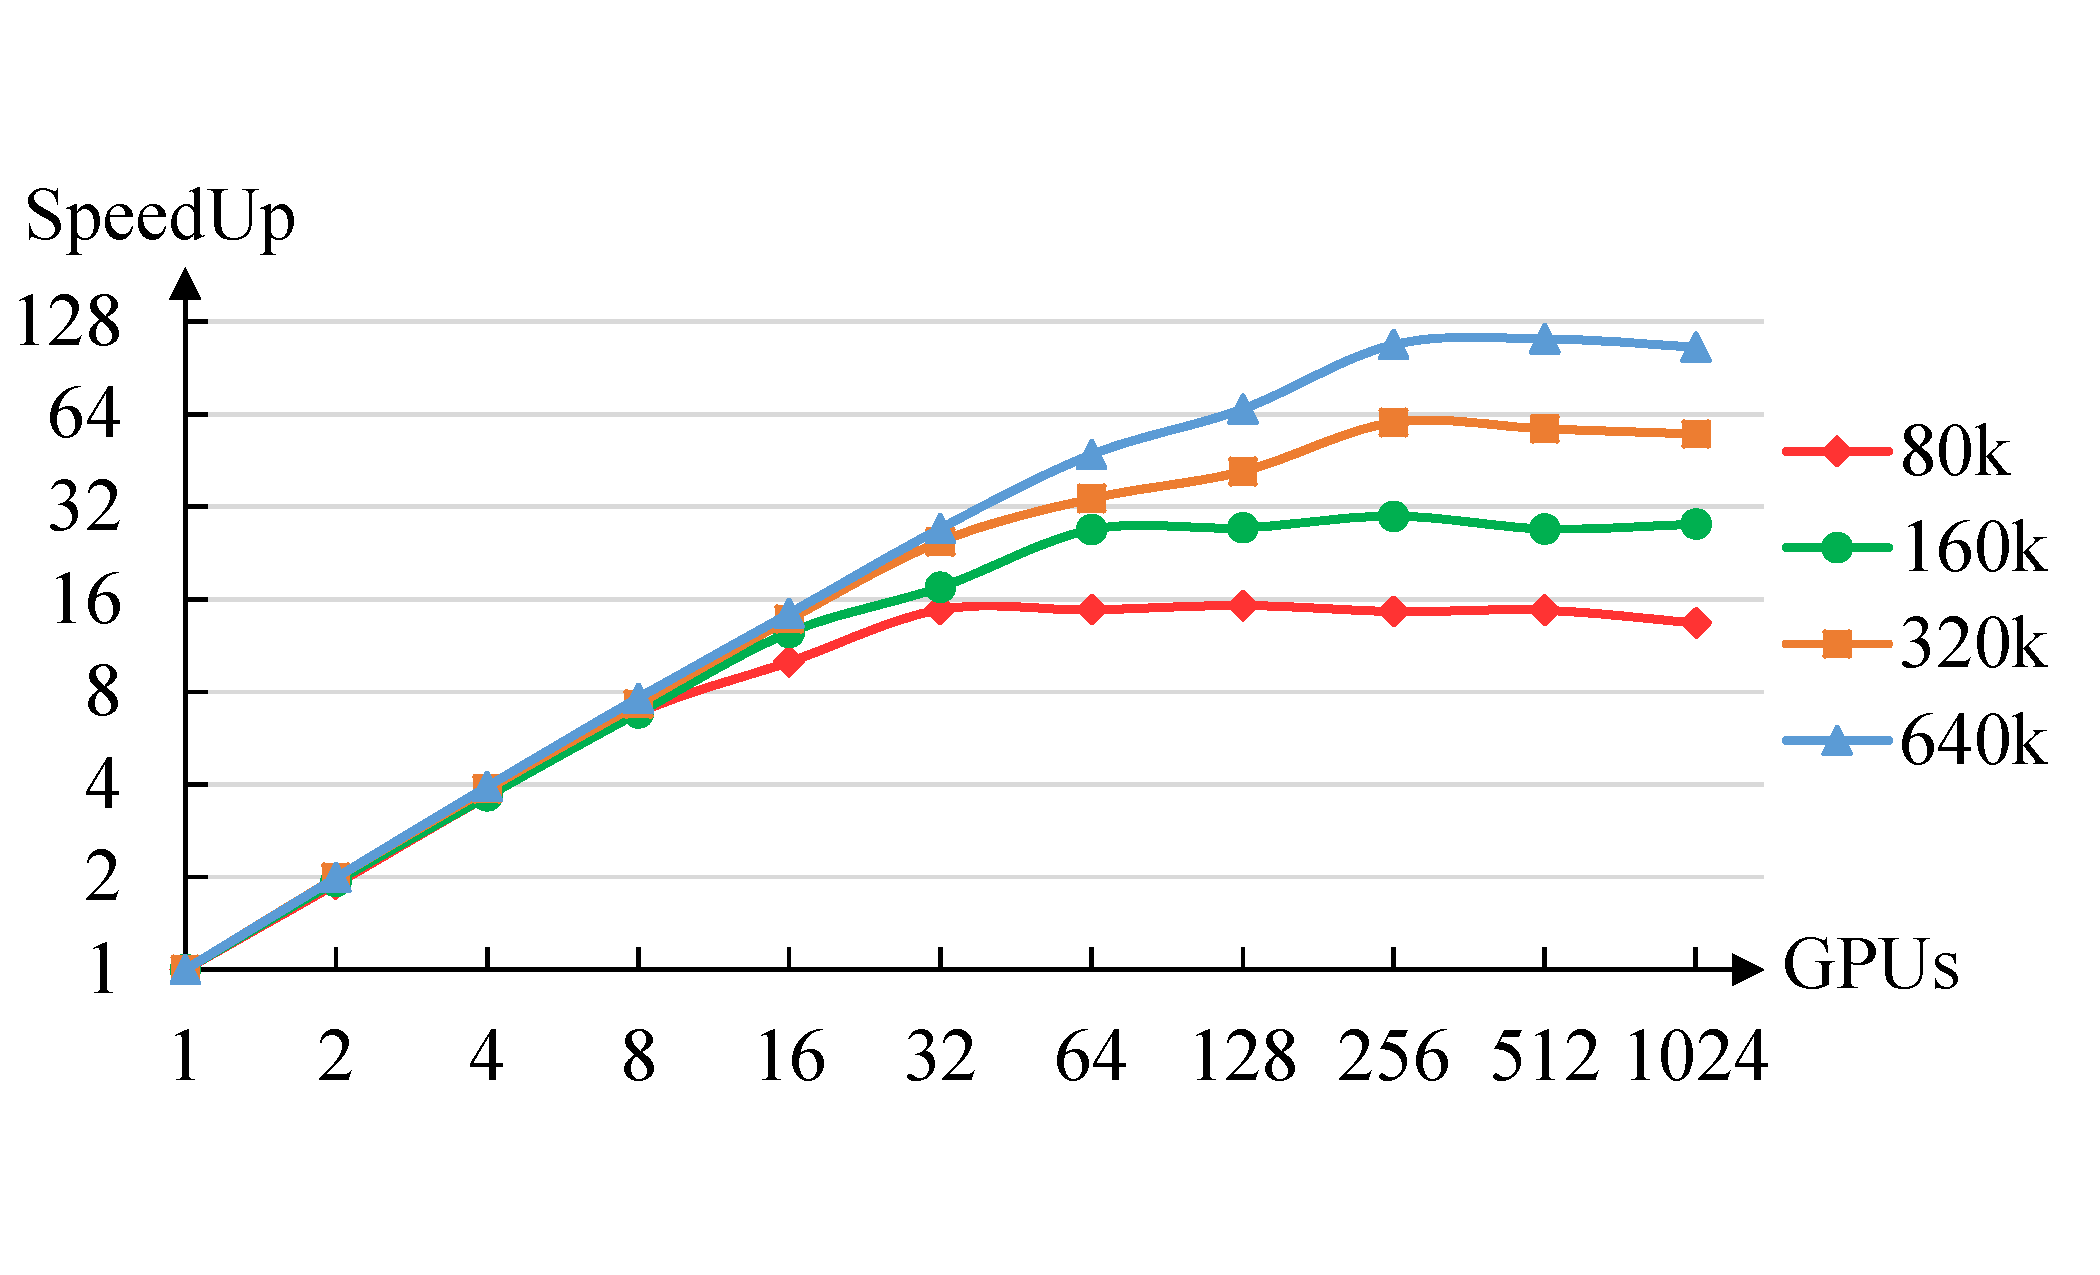
\includegraphics[width=\textwidth]{Img/640k_speedup_of_looptime5log.pdf}
        \caption{程序整体加速比}
        \label{fig:TotalTitan}
    \end{subfigure}
    \caption{多GPU加速比}\label{fig:Titan}
\end{figure}

由图\ref{fig:SCTitan}可得,在一开始,空间电荷效应求解器的加速比随着GPU的数目几乎线性增加,随后,加速比逐渐到达一个极限。
一方面,加速比的线性增长主要是因为GPU之间的数据交换量很少。这是无网格保辛粒子跟踪算法的一个很大的优势,其数据交换量仅与模式数量有关,而与粒子数量无关。
另一方面,它可以实现的最大加速度主要受粒子数量的限制,线性增加的范围和极限也随着粒子数量的增加而增加。以160000粒子为例,加速比最大可以达到40。在Titan集群上,每个GPU包含2688个内核,当使用64个GPU时,我们使用了64 $\times$ 2688 = 172032个内核,即使用的核心数多于粒子数。在这种情况下,我们无法通过简单地使用更多的GPU来获得进一步加速。而粒子数目增加时,比如320000个粒子或640000个粒子,所能够使用的GPU数目也会随之增加,最大加速比和线性范围也就会增加。

图\ref{fig:TotalTitan}是程序整体总时间的加速比,其中外部传输矩阵,坐标变换,粒子信息统计这些部分也是并行化的。但是因为它们的计算量较低,很难取得很高的并行度。所以加速比略微下降。

\section{三阶共振模拟}            \label{section:3rd_order_simulation}
我们使用Symplectic算法在周期聚焦结构中进行粒子跟踪和模拟。我们使零流强的周期相移为86.3259度,如果将10个周期视为一个环,则环的工作点为2.3979。随着流强的增加,相移会被压缩,工作点会在0.6A左右穿过2.3333的三阶共振线。环中还存在一个六极磁铁。

图\ref{fig:emitGrowthCompare}为不同流强下的束流发射度增长变化,可以看到,发射度在流强为0.1A 和0.2A 时基本保持不变,这时的工作点约为2.40。但是发射度在流强为0.4A,0.6A,和0.8A时持续增长,这时的工作点在2.3333附近,可知其发射度增长是由于三阶共振导致。

\begin{figure}[!htb]
    \centering
    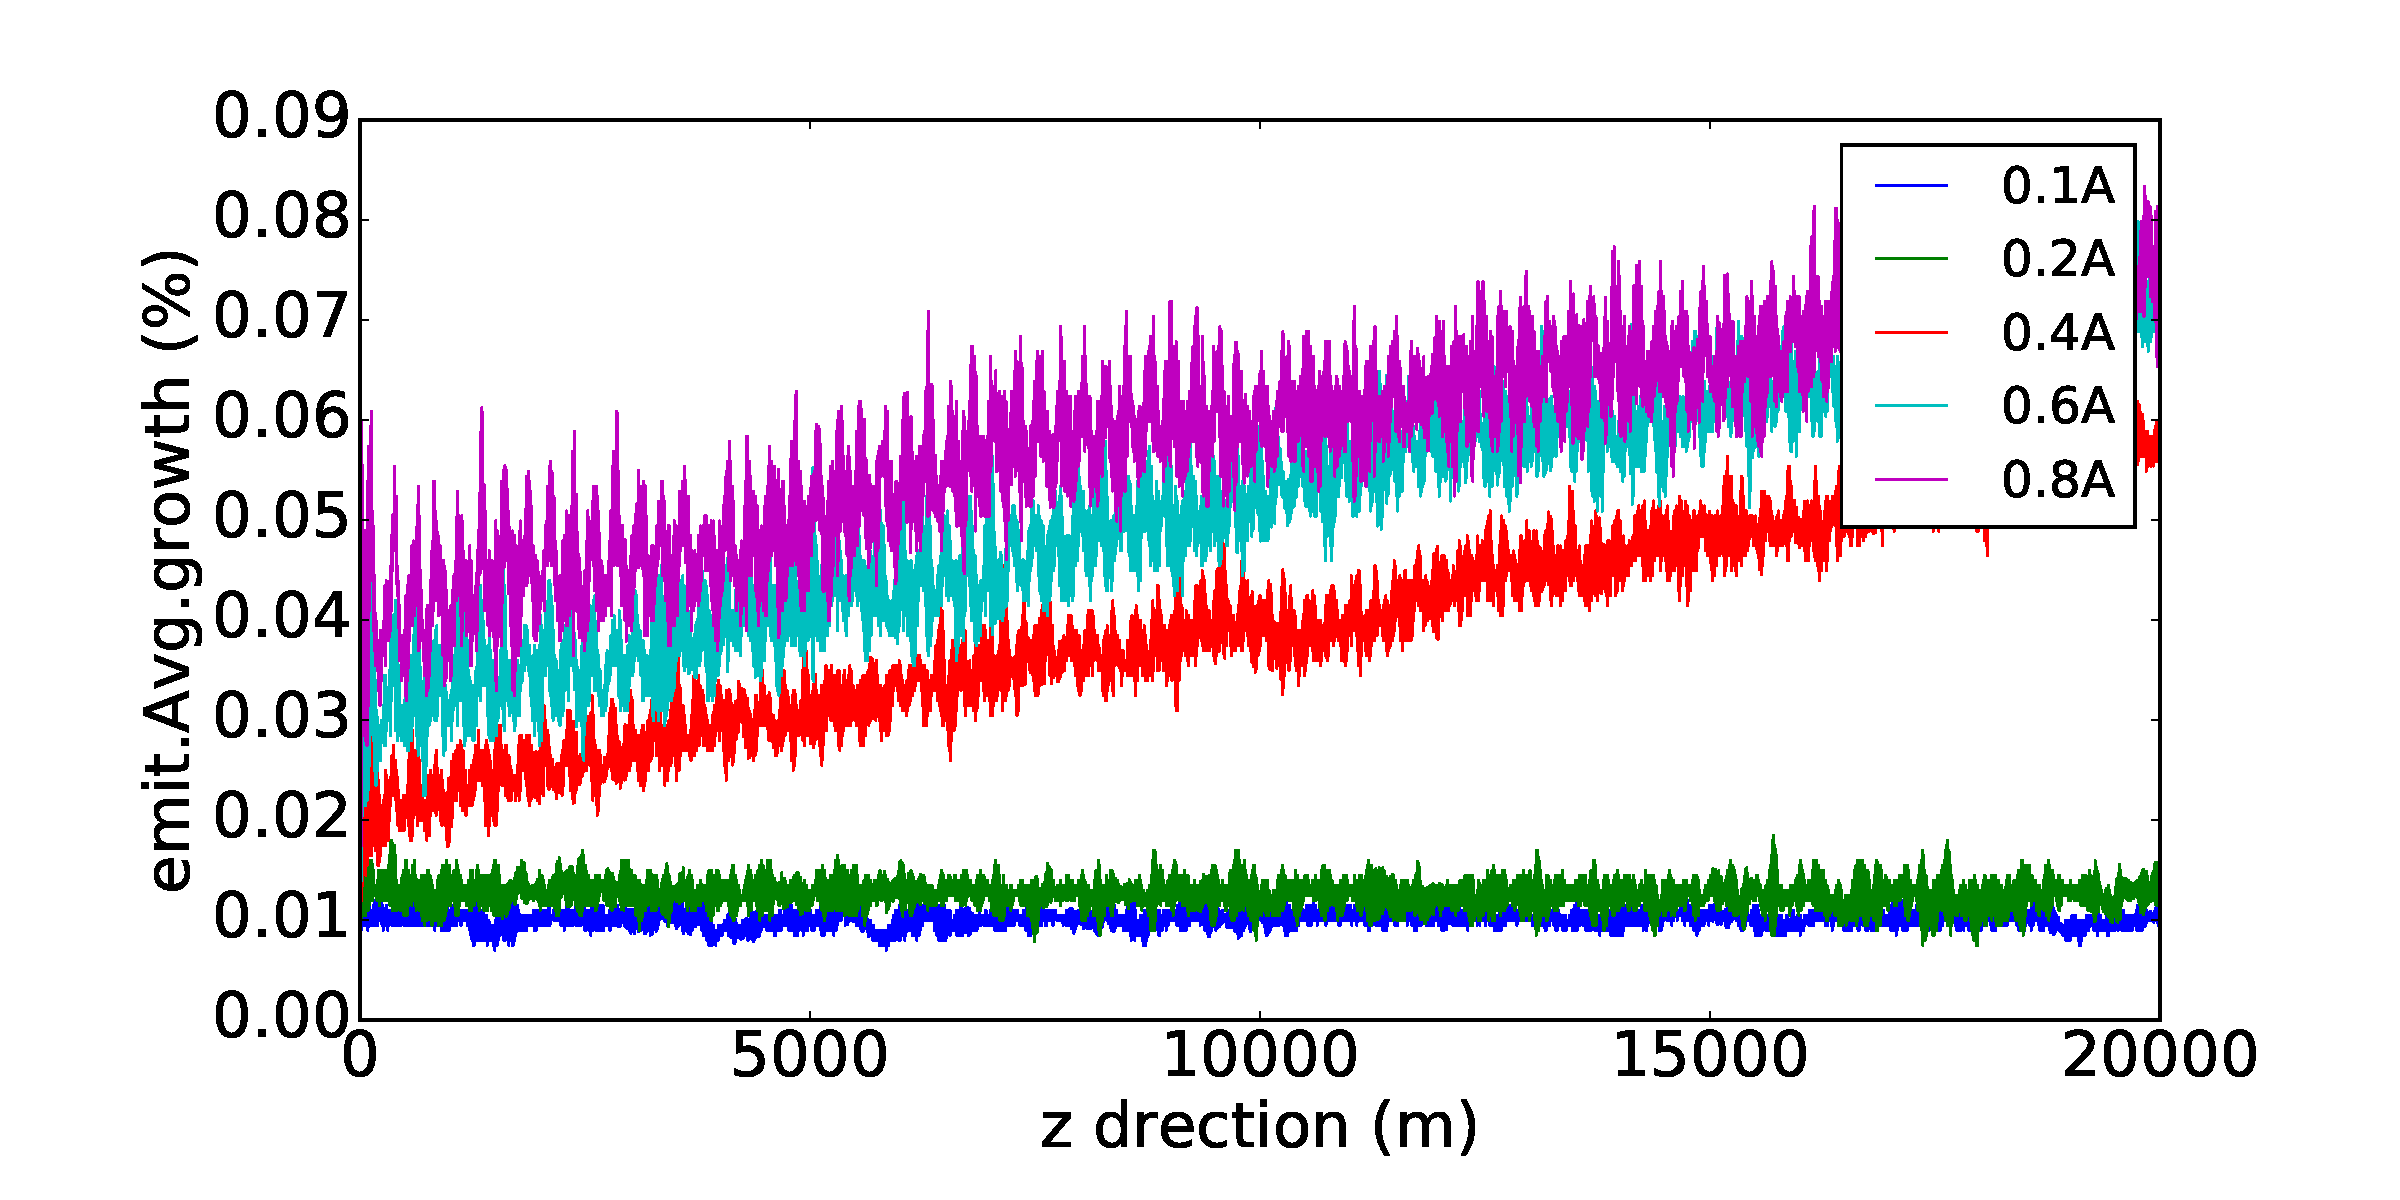
\includegraphics[width=0.95\textwidth]{Img/SymplecticEmitGrowthCompare.pdf}
    \caption{不同流强下的发射度增长}
    \label{fig:emitGrowthCompare}
\end{figure}

图\ref{fig:Poincare}是工作点为2.3333附近时的粒子坐标的庞加莱截面,其中颜色越暗表示粒子密度越大,而不同的图片代表粒子处于不同的初始位置。受空间电荷效应驱动,庞加莱截面会被被扭曲,并塑造成三角形形状。受到三阶共振影响的粒子的横向位置会逐渐变大。最后,粒子会成为束晕的一部分并丢失。

\begin{figure}[!htb]
    \centering
    \begin{subfigure}[b]{0.48\textwidth}
        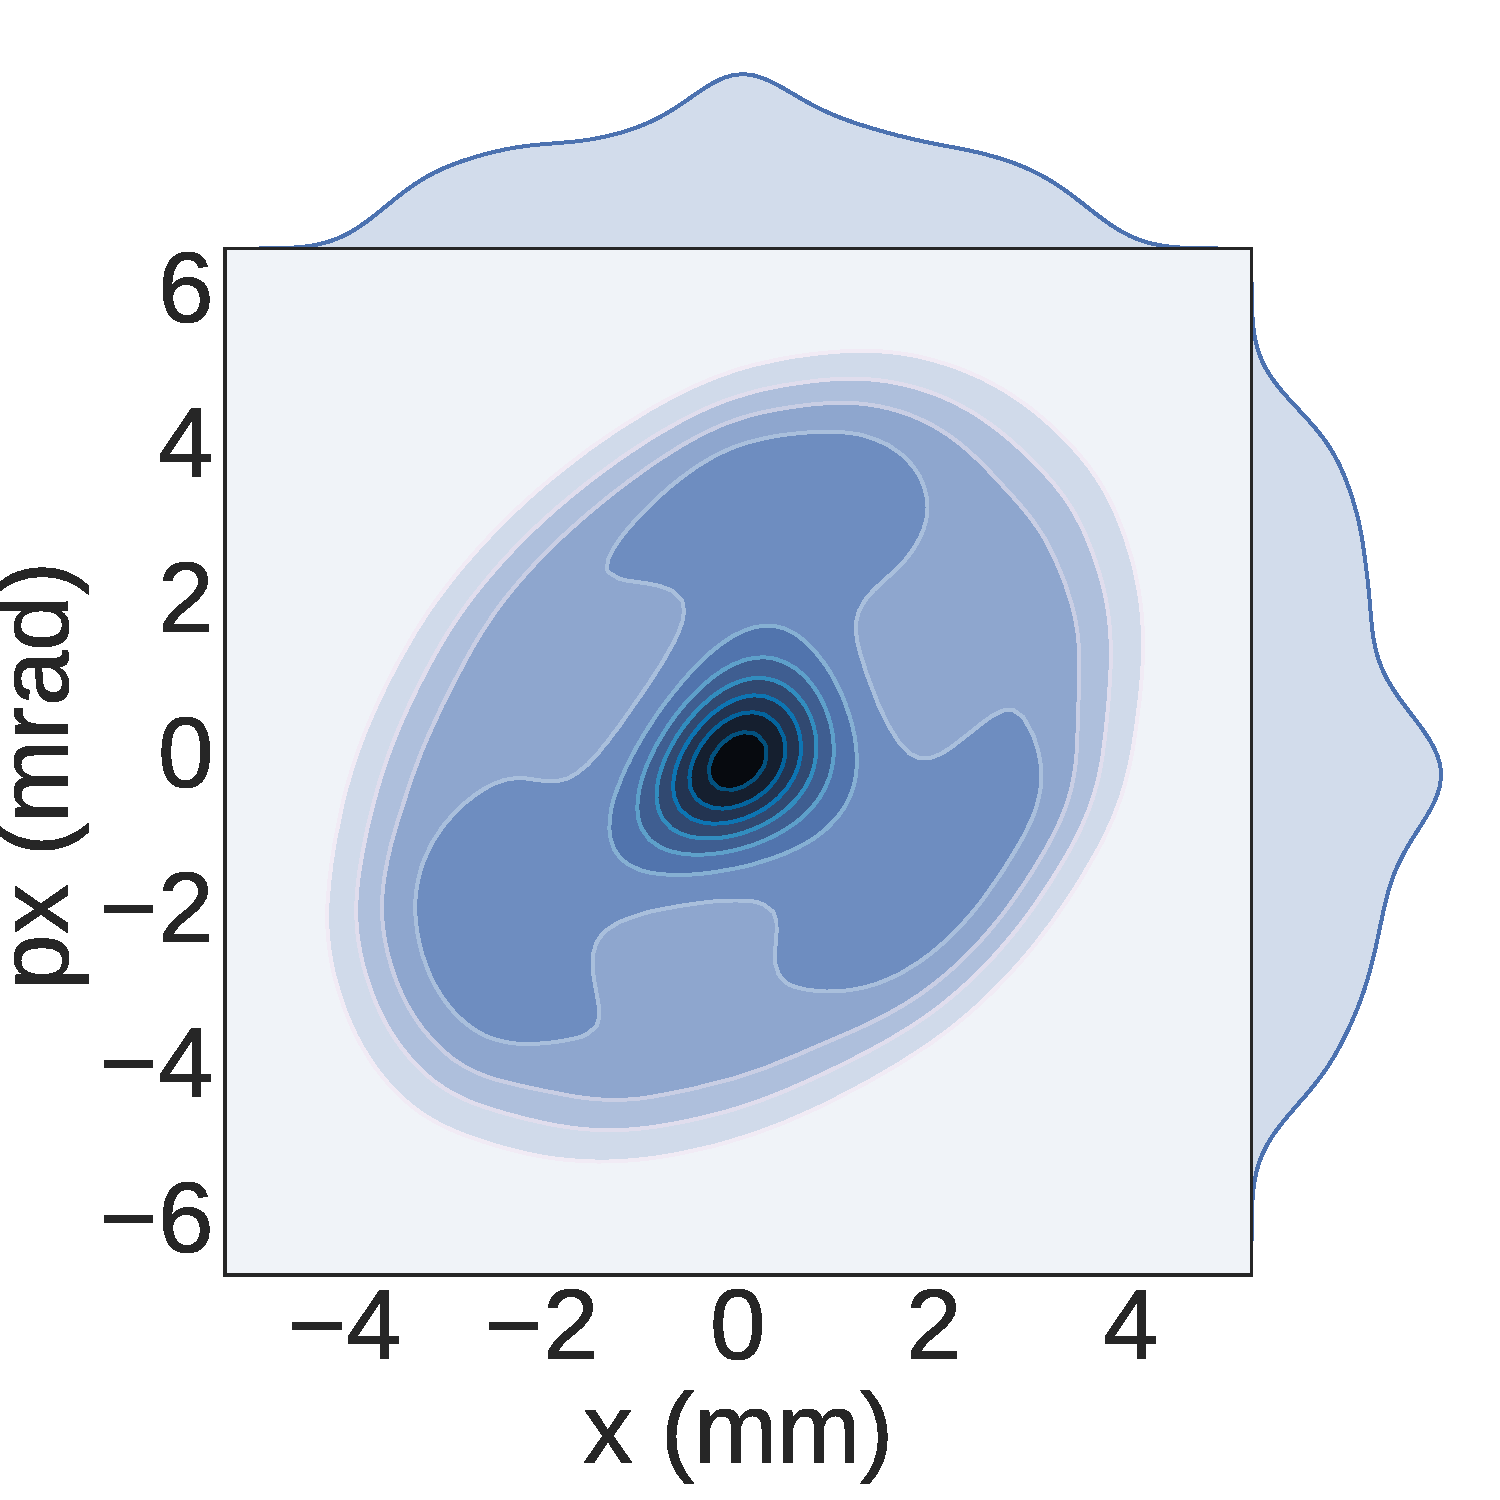
\includegraphics[width=\textwidth]{Img/particle_contour_nlevel9/sptc00002_xpx.pdf}
        \caption{}
    \end{subfigure}
    \begin{subfigure}[b]{0.48\textwidth}
        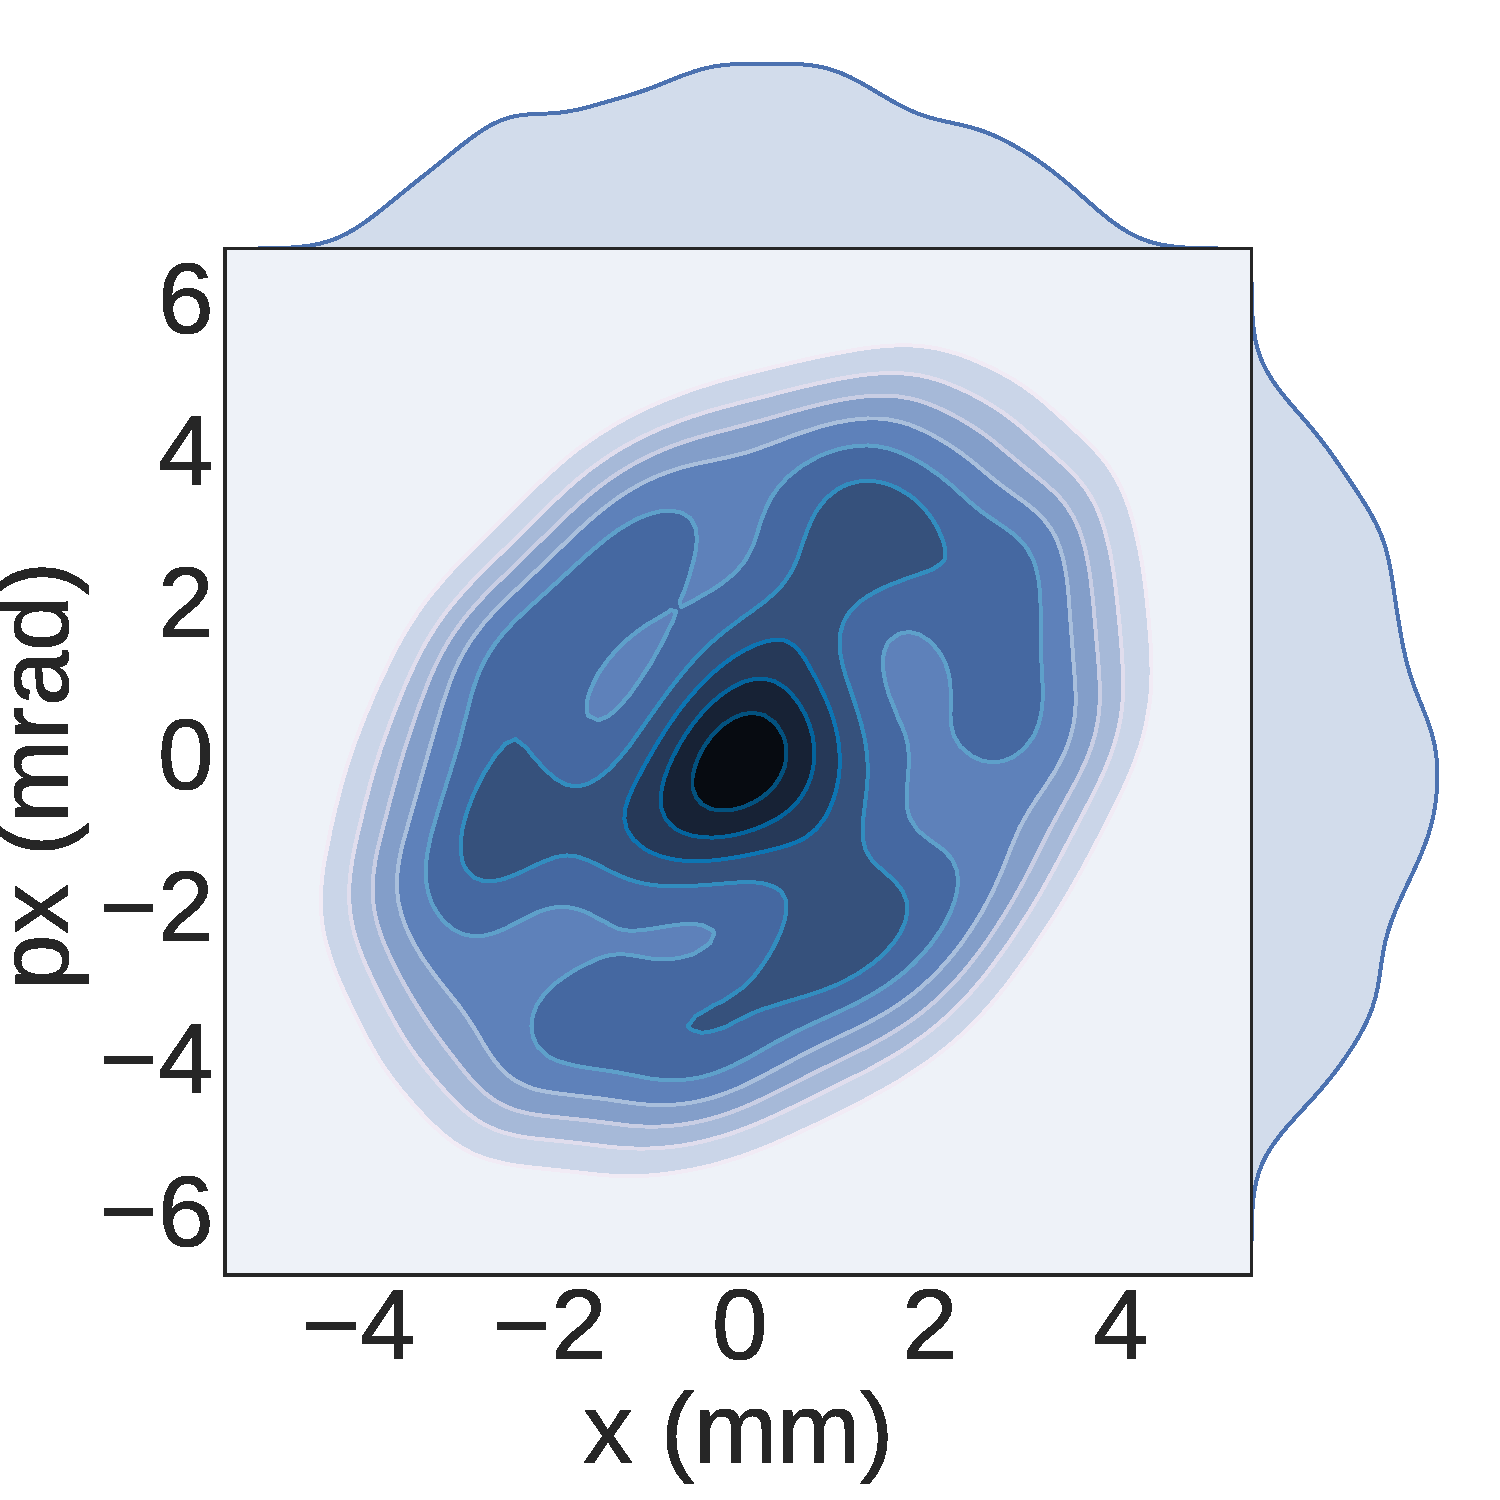
\includegraphics[width=\textwidth]{Img/particle_contour_nlevel9/sptc00005_xpx.pdf}
        \caption{}
    \end{subfigure}
    \begin{subfigure}[b]{0.48\textwidth}
        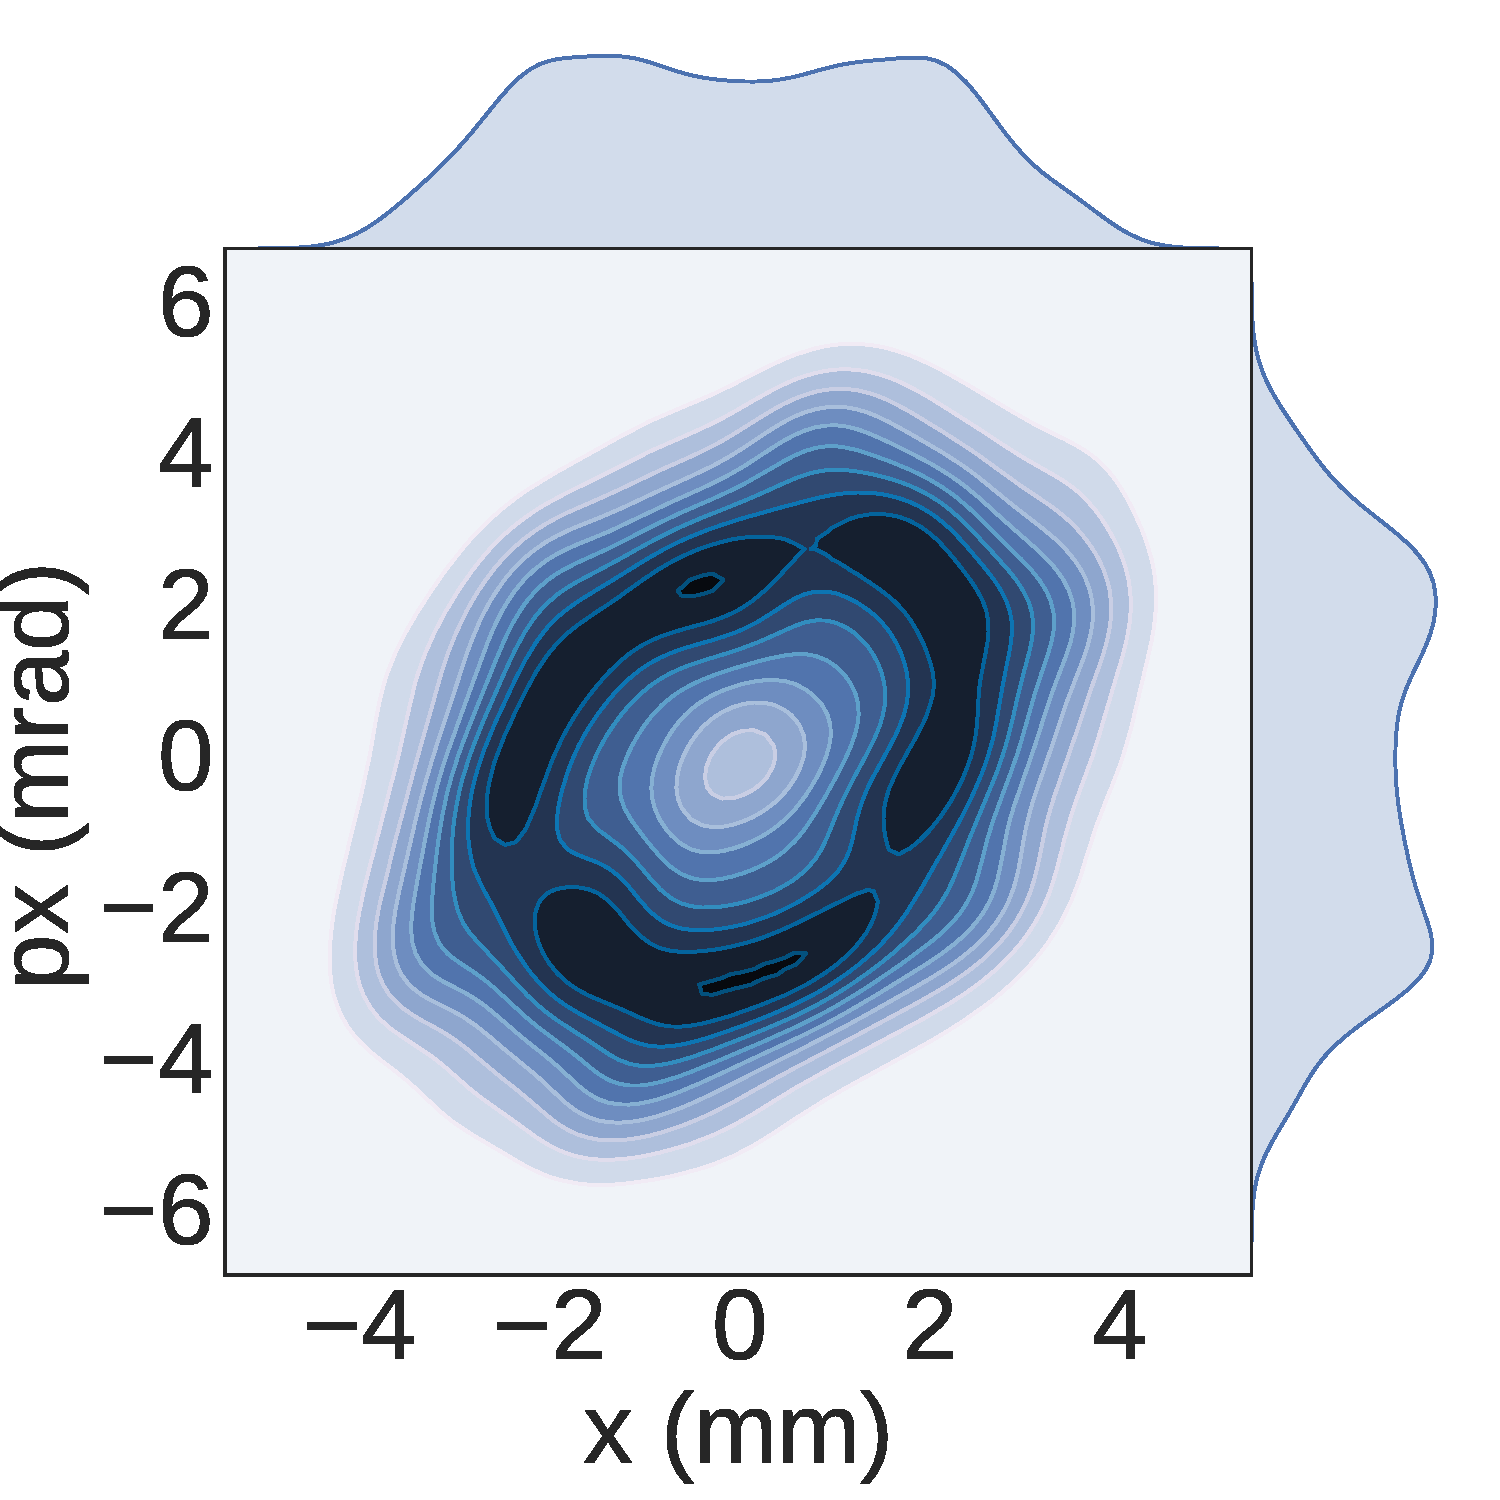
\includegraphics[width=\textwidth]{Img/particle_contour_nlevel9/sptc00003_xpx.pdf}
        \caption{}
    \end{subfigure}
    \begin{subfigure}[b]{0.48\textwidth}
        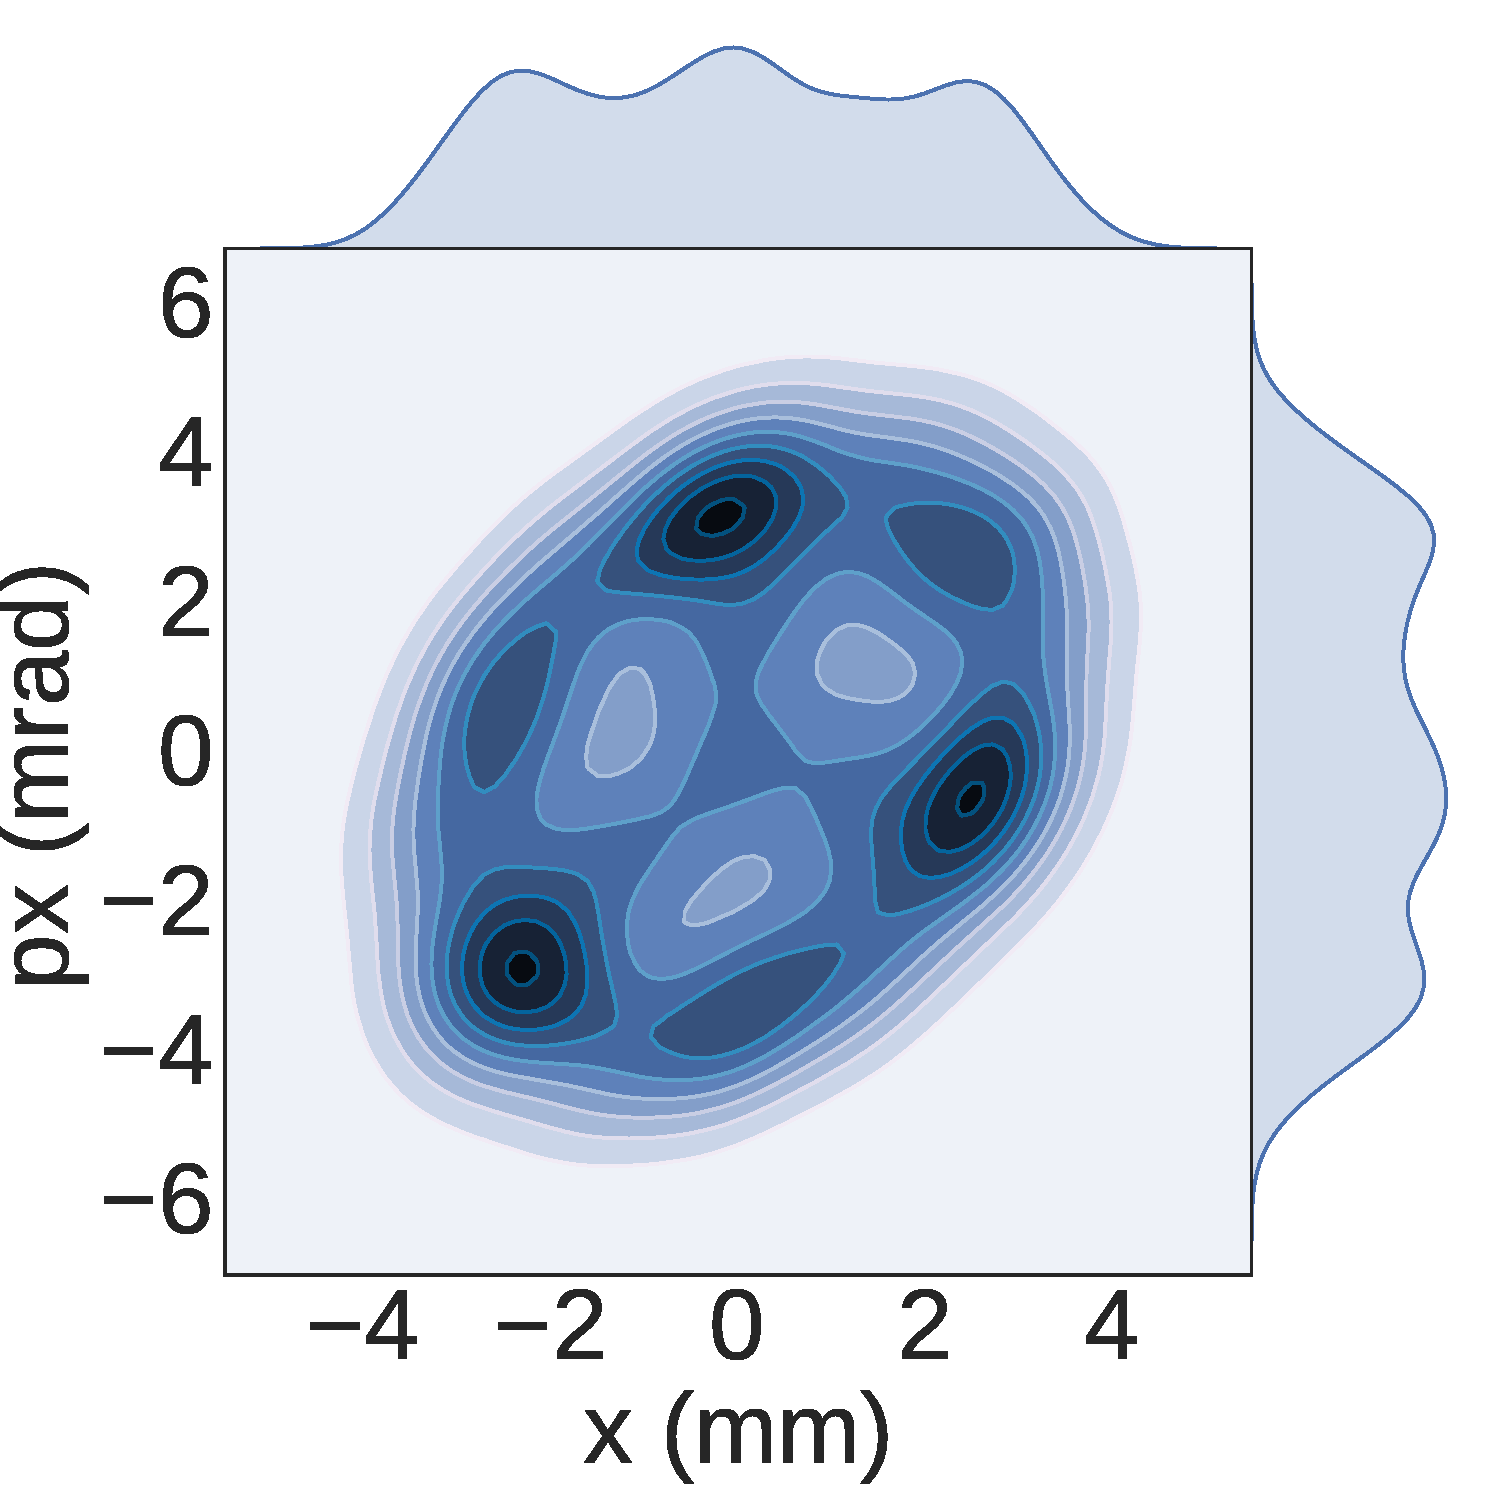
\includegraphics[width=\textwidth]{Img/particle_contour_nlevel9/sptc00006_xpx.pdf}
        \caption{}
    \end{subfigure}
    \caption{三阶共振附近的庞加莱截面}\label{fig:Poincare}
\end{figure}
\section{C-ADS注入器I模拟}        \label{section:ADS_simulation}
我们使用P-TOPO程序模拟了C-ADS的注入器I。C-ADS的注入器I由离子源(~electron cyclotron resonance ion-source, ECRIS),低能传输线,RFQ,中能传输线,两个超导加速模块,以及最后的垃圾桶组成,其结构如图\ref{fig:ADS_layout}所示

\begin{figure}[!htb]
    \centering
    
\includegraphics[width=0.99\textwidth]{Img/Layout_of_ADS_Injector_I.jpg}
    \caption{C-ADS注入器I结构示意图}
    \label{fig:ADS_layout}
\end{figure}

C-ADS注入器I的基本参数如表\ref{tab:C_ADS_parameters}所示。其中RFQ是使用PARMTEQM\cite{crandall1998rfq}设计的,频率为325MHz,将10mA的质子束流从35keV加速到3.2MeV,并且以后有可能升级到15mA。因为注入能量较低,只有35keV,RFQ的参数和聚束节使用绝热设计以降低空间电荷效应的影响,这导致了最终较小的纵向发射度。RFQ之后是超导加速腔,经过14个Spoke腔将束流加速到最终的10MeV。

\begin{table}[!htbp]
    \centering
    \footnotesize% fontsize
    \setlength{\tabcolsep}{4pt}% column separation
    \renewcommand{\arraystretch}{1.2}%row space
    \begin{tabular}{lc}
        \hline\hline
        Particle                & Proton \\
        \hline
        Rf frequency (MHz)      & 325       \\
        \hline
        Injection energy (MeV)  & 0.035     \\
        \hline
        Output energy (MeV)     & 10        \\
        \hline
        Pulsed beam current (mA)& 10        \\
        \hline
        Beam duty factor        & 100\%     \\
        \hline
        Input normalized rms emittance X ($\pi$ mm mrad)    & 0.2        \\
        \hline
        Input normalized rms emittance Y ($\pi$ mm mrad)    & 0.2        \\
        \hline\hline
    \end{tabular}
    \caption{C-ADS注入器I基本参数}
    \label{tab:C_ADS_parameters}
\end{table}

我们对RFQ和后面的超导段分别进行模拟,宏粒子数目为20000个,横向初始分布使用KV分布,纵向初始分布为均匀分布。使用实际运行的加速器结构,并且当粒子的横向位置触碰元件的孔径后标记为丢失,其中RFQ稍微严格对待,其孔径为当前cell的最小半径。空间电荷效应的网格数为64*64*64(x/y/z)。在RFQ段,我们不但使用P-TOPO程序,同时也使用Track程序\cite{aseev2005track},以相同的初始条件进行模拟;同样的,在超导段,除了P-TOPO之外,我们还使用TraceWin\cite{uriot2014tracewin}来进行研究和对比。下面,我们对RFQ和超导段分别进行讨论。

\subsection{RFQ模拟}
在RFQ模拟中,RFQ中的场可由傅里叶贝塞尔方程的八项式得到,如式\ref{eq:RFQ_8terms}:
\begin{equation}
    \begin{aligned}
       {{U}_{ex}}(r,\theta ,z) & =\frac{V}{2}[{{A}_{01}}{{(r/{{r}_{0}})}^{2}}\cos (2\theta )+{{A}_{10}}{{I}_{0}}(kr)\cos (kz) \\
     & +{{A}_{03}}{{(r/{{r}_{0}})}^{6}}\cos (6\theta )+{{A}_{21}}{{I}_{2}}(2kr)\cos (2\theta )\cos (2kz) \\
     & +{{A}_{12}}{{I}_{4}}(kr)\cos (4\theta )\cos (kz)+{{A}_{03}}{{I}_{0}}(3kr)\cos (3kz) \\
     & +{{A}_{23}}{{I}_{6}}(2kr)\cos (6\theta )\cos (2kz)+{{A}_{32}}{{I}_{4}}(3kr)\cos (4\theta )\cos (3kz)]
    \end{aligned}
    \label{eq:RFQ_8terms}
\end{equation}
其中$I_n$为第n阶修正贝塞尔方程,$k=\pi /2\beta \gamma$,$A_mn$系数由RFQ设计程序PARMTEQM给出。

图\ref{fig:ADS_RFQ_emit}是P-TOPO和TRACK在0mA下和15mA下对RFQ模拟得到的横向和纵向发射度演化,其中红色实线为P-TOPO的结果而绿色虚线为TRACK的结果。在横向和纵向两个方向上,P-TOPO的发射度演变结果都更加光滑,尤其是在RFQ的前端。在此处,束流开始丝化形成束团,并且相空间开始剧烈旋转。P-TOPO与TRACK的结果误差在合理范围内。

\begin{figure}[!htb]
    \centering
    \begin{subfigure}[b]{0.9\textwidth}
        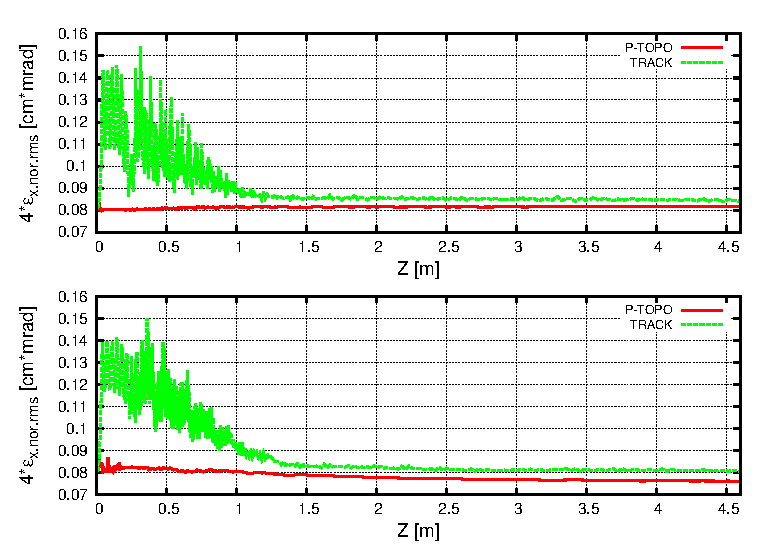
\includegraphics[width=\textwidth]{Img/ADS_RFQ_emit1.eps}
        \caption{0mA(上)和15mA(下)时RFQ中的横向发射度}
    \end{subfigure}
    \begin{subfigure}[b]{0.9\textwidth}
        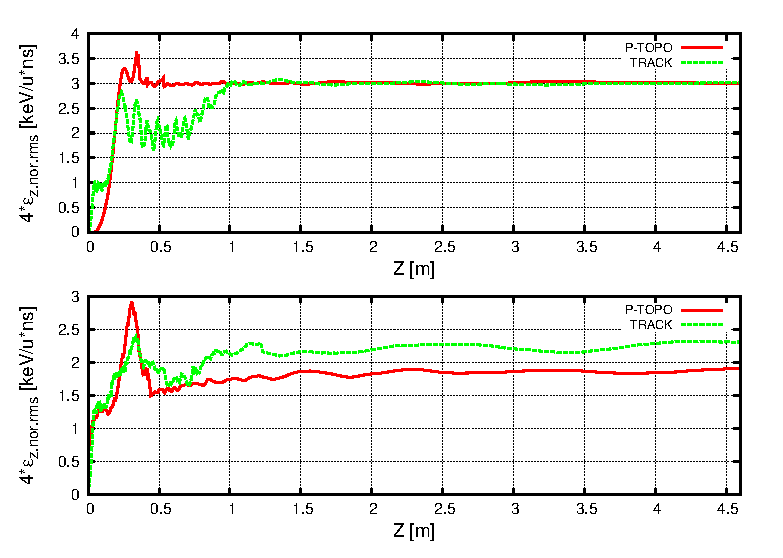
\includegraphics[width=\textwidth]{Img/ADS_RFQ_emit2.eps}
        \caption{0mA(上)和15mA(下)时RFQ中的纵向发射度}
    \end{subfigure}
    \caption{RFQ中的横向发射度和纵向发射度}\label{fig:ADS_RFQ_emit}
\end{figure}


图\ref{fig:ADS_RFQ_size1}是P-TOPO和TRACK在15mA下对RFQ模拟得到的横向束团尺寸演化,图~\ref{fig:ADS_RFQ_size2}是~P-TOPO和TRACK在15mA下对RFQ模拟得到的纵向束团尺寸和能散演化,其中红色实线为P-TOPO的结果而绿色虚线为TRACK的结果。两个程序在束团均方根尺寸上吻合得很好,其差别在合理范围内。同时验证了C-ADS注入器I的RFQ设计能够有效的控制束团的发射度和尺寸。

\begin{figure}[!htb]
    \centering
    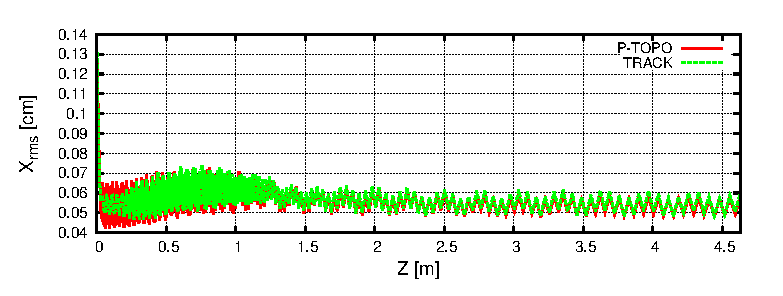
\includegraphics[width=0.9\textwidth]{Img/ADS_RFQ_size1.eps}
    \caption{RFQ中束团横向均方根尺寸}
    \label{fig:ADS_RFQ_size1}
\end{figure}

\begin{figure}[!htb]
    \centering
    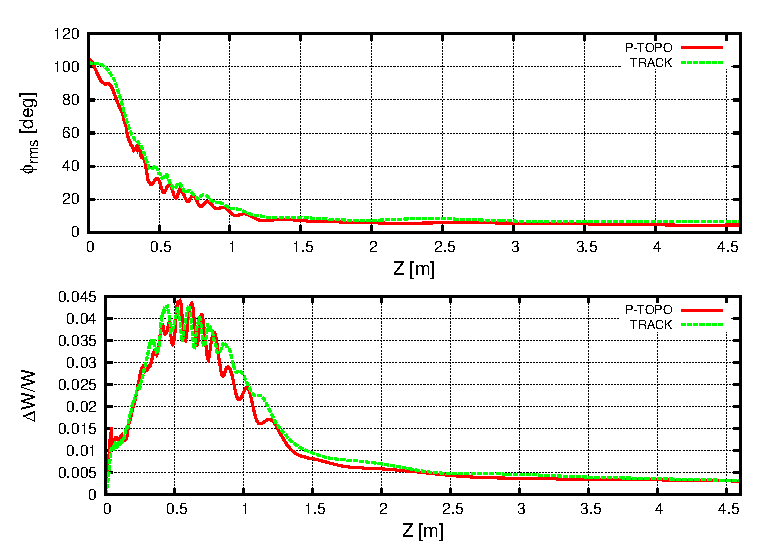
\includegraphics[width=0.9\textwidth]{Img/ADS_RFQ_size2.eps}
    \caption{RFQ中束团纵向均方根尺寸和能散}
    \label{fig:ADS_RFQ_size2}
\end{figure}

\subsection{超导段模拟}
在超导段中,聚束腔和加速腔的场由文件导入,P-TOPO使用数值差值来得到粒子所受到的场强。在设计的15mA流强下,RFQ出口处3.2MeV的质子束流经过聚束,通过MEBT进入超导段,逐渐加速到10MeV。在超导段中我们使用P-TOPO和~TraceWin来进行模拟。

图\ref{fig:ADS_SC_emit}为P-TOPO和TraceWin在15mA下对RFQ模拟得到的横向和纵向发射度演化,其中红色实线为P-TOPO的结果而绿色虚线为TraceWin的结果。
两个程序得到的结果相一致。其中横向发射度除了在螺线管处有一个峰值外,基本保持不变。螺线管处的峰值是因为P-TOPO和TraceWin都是以时间t为基本变量,即发射度是由同一时刻的粒子信息统计得到,而不是由同一纵向位置的粒子得到,因此,在束团进入螺线管的时候,部分粒子先进入,部分粒子还没有进入,导致相空间的扭曲,从而导致统计发射度的突变。纵向发射度有略微增长,增长幅度在20\%以内。横纵向的发射度增长是由空间电荷力,磁铁边缘场的非线性效应,以及超导腔内的非线性纵向力导致,这几个驱动发射度增长的来源共同作用,使粒子相空间扭曲,最终会导致束晕的产生。P-TOPO的模拟中,出口能量为10.01MeV,而TraceWin的模拟出口能量为10.06MeV。
\begin{figure}[!htb]
    \centering
    \begin{subfigure}[b]{0.9\textwidth}
        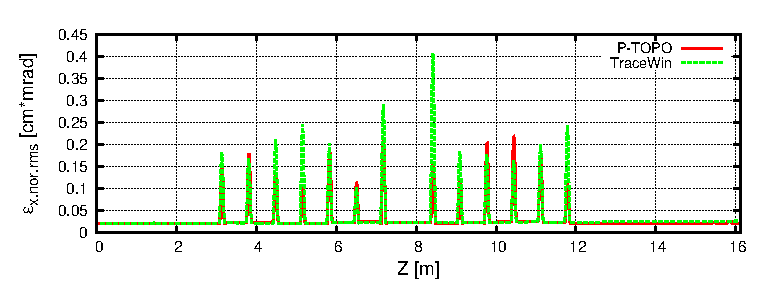
\includegraphics[width=\textwidth]{Img/ADS_SC_emit1.eps}
        %\caption{}
    \end{subfigure}
    \begin{subfigure}[b]{0.9\textwidth}
        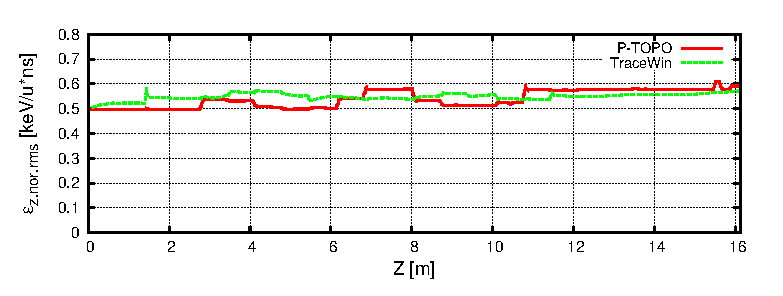
\includegraphics[width=\textwidth]{Img/ADS_SC_emit2.eps}
        %\caption{}
    \end{subfigure}
    \caption{超导段横向发射度和纵向发射度}\label{fig:ADS_SC_emit}
\end{figure}

图\ref{fig:ADS_SC_size}是P-TOPO和TraceWin在15mA下对超导段模拟得到的横纵向束团尺寸演化和能散演化,其中红色实线为P-TOPO的结果而绿色虚线为TRACK的结果。两个程序模拟结果的细微差别主要是因为两个程序获取同步相位的方法不同。~TraceWin使用时间漂移法获得同步相位,而P-TOPO使用扫相获得同步相位。束团的横向尺寸相比管道半径都很小,而纵向尺寸也被聚束腔和接下来的各个加速腔有效地压缩,一般不会有束损出现。
\begin{figure}[!htb]
    \centering
    \begin{subfigure}[b]{0.9\textwidth}
        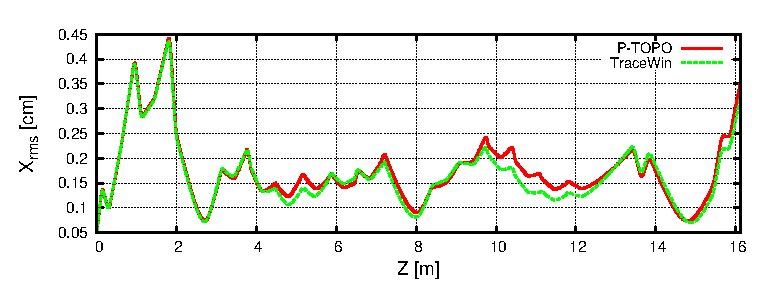
\includegraphics[width=\textwidth]{Img/ADS_SC_size1.eps}
        %\caption{}
    \end{subfigure}
    \begin{subfigure}[b]{0.9\textwidth}
        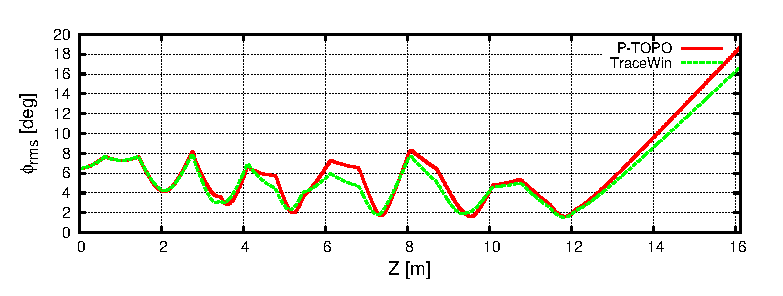
\includegraphics[width=\textwidth]{Img/ADS_SC_size2.eps}
        %\caption{}
    \end{subfigure}
    \begin{subfigure}[b]{0.9\textwidth}
        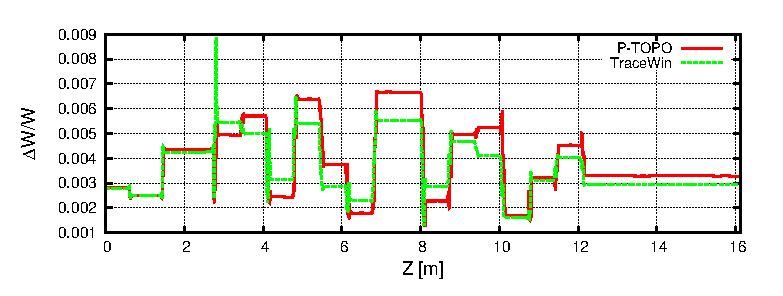
\includegraphics[width=\textwidth]{Img/ADS_SC_size3.eps}
        %\caption{}
    \end{subfigure}
    \caption{超导段束团横纵向尺寸以及能散}\label{fig:ADS_SC_size}
\end{figure}

在RFQ和超导段两段模拟中,传输效率都在99.9\%以上,束团尺寸和束损都得到了有效控制,横向和纵向的发射度都保持良好。不同代码的模拟结果差别主要是因为初始的束团分布不同,以及统计数据的方式不同,特别是P-TOPO是以时间t为基本变量,而TRACK是以位置z为基本变量,因此粒子信息收集,空间电荷力的计算,以及粒子推动方式都有所不同。

\section{共振穿越研究}

加速器中的非线性束流动力学已经在数值和实验上进行了很多年的研究~\cite{accelerator2004lee,reiser2008theory}。
如今,加速中由各种非线性机制驱动产生的的共振被认为是导致束流恶化的主要来源,例如束流RMS发射度增长、束晕、束损。
一般来说,对束流动力学行为的研究是在哈密顿系统的框架中进行的,而粒子哈密顿系统中的非线性项可以视为微扰,这样共振条件就可以使用线性微扰理论来得到。
除了由于正常的加速器元件产生的非线性之外,束团内部的空间电荷效应是另外一个主要来源。
并且,在强流质子加速器中,空间电荷效应会在不同自由度之间产生耦合,我们必须对其仔细处理~\cite{accelerator2013chao}。

束流运动的非线性共振可以分两个层次来进行描述:单粒子动力学(非相干效应)和RMS束流动力学(相干效应)。
单粒子动力学描述的一个典型例子是共振线图中由于加速器中多级铁和Lattice的误差导致的各阶共振线$n\nu_x+m\nu_y$。
共振线图被广泛应用在加速器的工作点选择和实际运行中。
考虑到非线性效应,工作点会产生偏移~\cite{fedotov2001space},
所以当束流工作点靠近共振线时就会发生单粒子周期共振穿越~\cite{franchetti2006particle}。
对于RMS束流动力学描述,外部元件和内部空间电荷效应产生的非线性效应在束流集体不稳定性中起到了非常关键的作用
\cite{sacherer1968transverse, sacherer1973longitudinal},
其可以通过以自洽的方式求解扰动的Vlasov方程来描述\cite{chao1993physics,gluckstern1970oscillation,gluckstern1970stability}。
然而,虽然人们付出了极大地努力来扩展这些模型以涵盖各种束流条件,但是我们仍然无法求得这种系统的解析解,可解决的问题只是局限于某些特定的情况。

对于强流离子束流中的空间电荷效应导致的集体不稳定性,其研究一方面从RMS包络方程出发~\cite{sacherer1971rms},
其中二阶不稳定性,即束流包络不稳定性,得到了人们广泛而深入的研究 ~\cite{14,15,16,17,21,22}。
而另一方面的研究从自洽的求解Vlasov-Poisson方程出发 ~\cite{11,12,18,19}。
研究表明,求解Vlasov-Poisson方程得到的二阶偶共振正是包络方程的得到的相干共振。
最近研究提出了一种空间电荷物理中的Vlasov-Poisson模型的通用理论~\cite{11, 12}。
其理论预测了在Lattice参数没有被精心优化的情况下,结构共振会伴随构造本征模式发生,
另外,低阶的结构共振禁带可以自然的作为高阶结构共振禁带的一部分\footnote{数学证明详见参考文献~\cite{12}}。

在一个实际的加速器中,外部元件的聚焦强度一般随着束流被加速而逐渐变化,其有可能导致“结构共振穿越”。
本节将重点介绍束流穿过结构共振禁带时,束流和粒子的相干和非相干特性将如何发展。
作为对Vlasov-Poisson模型的理论研究的延伸,我们选取了$90^{\circ}$相移附近的的二阶共振禁带进行研究,并使用PIC模拟来验证了理论预测的有效性。这些研究可以很容易地扩展到更高阶的模式,比如三阶($60^{\circ}$)和六阶结构共振($120^{\circ}$)~\cite{36,40}。
需要注意的是,束流和结构共振之间的相互作用必须以瞬态进行研究。
而低阶相干模是高阶模的组成部分是理解在模拟和实验结果的关键~\cite{groening2009experimental,33}。

第\ref{section:Crossing_model}节简要介绍了结构共振模型,并定义了用来描述相干和非相干效应的一些术语。
第\ref{section:Crossing_Coherent}节中给出了禁带的方程,使用多粒子PIC追踪程序模拟了束流穿越相干结构共振时的现象,并在暂态意义上进行了讨论。第\ref{section:Crossing_Incoherent}节讨论了非相干共振的粒子特征。
最后第\ref{section:Crossing_Summary}节进行了总结。

\subsection{物理模型}
\label{section:Crossing_model}
本节简要介绍了结构共振的物理模型和基本的处理方法,其中可解的耦合~Vlasov-Poisson方程仅限于4D KV分布~\cite{20}。

接下来,我们使用周期性的FODO结构来模拟加速器中的连续束的演变, 考虑到周期聚焦结构中完全匹配的束流的哈密顿量是恒定的,平衡分布函数可以表示为哈密顿量:
\begin{eqnarray}\label{eq2.1}
  f_0(x,p_x,y,p_y) =f(H_0),  \quad  H_0&=&k_x(s)x^2+p_x^2+k_y(s)y^2+p_y^2+V_{sc}(x,y)
\end{eqnarray}
其中 $k_x(s)$和$k_y(s)$外部四级铁的聚焦强度, $V_{sc}(x,y)$是空间电荷势。分布函数 $f_0$必须同时满足Vlasov方程和 Poisson方程:
\begin{eqnarray}\label{eq2.2}
\frac{\partial f_0}{\partial s} + [f_0,H_0]=0,   \quad \Delta V_{sc}(x,y)  = \frac{1}{\epsilon_0}  \int \int f_0 dxdy,
\end{eqnarray}
其中 $[,]$为泊松括号。

如果粒子分布函数存在一个扰动 $f_1$,其将会导致空间电荷势受到扰动$V_1=H_1$.。这样,一阶线性Vlasov方程和Poisson方程可以表示为:
\begin{eqnarray}\label{eq2.3}
\frac{\partial f_1}{\partial s} + [f_1,H_0] +  [f_0,V_1]=0,   \quad \Delta V_1(x,y)  = \frac{1}{\epsilon_0}  \int \int f_1 dxdy.
\end{eqnarray}
这组方程只有在粒子分布为理想的KV分布$f_0=\delta(H_0)$的时候才可解。一般情况下,束流内受扰动的空间电荷势可以表示为多项式的形式:
\begin{eqnarray}\label{eq2.4}
V_1=\sum_{m=0}^{n}A_m(s)x^{n-m}y^m +\sum_{m=0}^{n-2}A_m^{(1)}(s)x^{n-m}y^m+\cdots.
\end{eqnarray}
集体模$I_{j;k,l}(s)$可以在适当的边界条件下得到。对于式~\ref{eq2.4}中的$n$阶偶数模和奇数模可以根据$m$是偶数或奇数来分开处理,其直接代表了粒子在实空间中的椭圆分布的形状和倾角。设 $S$为一个聚焦周期的长度,集体模$I_{j;k,l}(s)$ 将满足$I'(s) = M(S)I(s)$,这正是$Mathieu$方程。而这个系统的稳定性将由其雅克比矩阵$M(S)$的本征值$\lambda$决定,详细的数学证明见参考文献~\cite{11,12,18,19}。

根据之前的研究\cite{11,12},结构共振条件可以显式的表达为$\Phi_{j;k,l}+\Phi_{j;k,l}=n\times 360^{\circ}$和$\Phi_{j;k,l}/\Phi_{e}=n/m$,其中$\Phi_{j;k,l}$为集体模$I_{j;k,l}$的本征相位;$\Phi_{e}$是一个周期中的包络震荡相移,恒为$360^{\circ}$。结构共振会随着本征相位锁定的现象发生,而发生结构共振的参数空间被称为不稳定禁带。

\subsection{结构共振穿越 -- 相干效应}
\label{section:Crossing_Coherent}
在加速器设计与运行中,有一条经验准则:“如果共振穿越不可避免,则穿越速度应该越快越好。”
比如在一些直线加速器的设计中,一开始的零流强相移大于$90^{\circ}$,之后在几个周期之内迅速降到 $90^{\circ}$以下。
接下来,我们使用$90^{\circ}$相移附近的二阶结构共振来研究当穿越共振禁带时的束流和结构共振之间的相互作用。
\footnote{如上文说述,二阶集体模实际上是四阶集体模的一部分~\cite{12},所以在下文中二阶模指的是二阶/四阶混合禁带。}
为了简化,我们使束流在两个方向上的发射度相等,并使用对称的周期FODO聚焦结构($k_x=k_y$)。

\subsubsection{二阶集体效应}
对于二阶偶数模,束流边界内部的扰动的空间电荷势为 $V_{2e}=A_0(s)x^2+A_2(s)y^2$;
对于二阶奇数模,其为 $V_{2o}=A_1(s)xy$。
动力学系统 $I'(s)=M(s)I(s)$ 可以得到 $(I_{0;2,0}, I_{2;0,2})$ 和  $(I_{1;1,1}, I_{1;1,-1})$ ,分别代表二阶偶数模和奇数模~\cite{11, 12, 18}。
其雅克比矩阵$M(s)$可以表示为:
\begin{eqnarray}\label{eq2.5}
M(s)=
\left(
  \begin{array}{cccc}
    0         & 1         & 0         & 0         \\
    J_{21}(s) & J_{22}(s) & J_{23}(s) & 0         \\
    0         & 0         & 0         & 1         \\
    J_{41}(s) & 0         & J_{43}(s) & J_{44}(s) \\
  \end{array}
\right).
\end{eqnarray}
上式中每个元素$J_{ij}(s)$的显式表达见附录~\ref{appdendix:Jacobi}.

\begin{figure}
    \centering
    \begin{subfigure}[b]{0.48\textwidth}
        \includegraphics[width=\textwidth]{Img/evenDepressedAbs.pdf}
        \caption{}
        \label{sfig:stopbandEvenAbs}
    \end{subfigure}
    \begin{subfigure}[b]{0.48\textwidth}
        \includegraphics[width=\textwidth]{Img/oddDepressedAbs.pdf}
        \caption{}
        \label{sfig:stopbandOddAbs}
    \end{subfigure}

    \begin{subfigure}[b]{0.48\textwidth}
        \includegraphics[width=\textwidth]{Img/evenDepressedArg.pdf}
        \caption{}
        \label{sfig:stopbandEvenArg}
    \end{subfigure}
    \begin{subfigure}[b]{0.48\textwidth}
        \includegraphics[width=\textwidth]{Img/oddDepressedArg.pdf}
        \caption{}
        \label{sfig:stopbandOddArg}
    \end{subfigure}
    \caption{二阶偶数模和奇数模的本征值 $Abs[\lambda_{j;k,l}]$ 和本征相位 $\Phi_{j;k,l}$ 随压缩相移 $\sigma$ 的变化}
    \label{fig:stopband}
\end{figure}

从包络方程出发的包络不稳定性非常有名,其描述了和二阶偶数模相同的物理机制~\cite{11,12,18}。
最近,人们使用Chernin模型研究了“和共振”与“差共振”不稳定性~\cite{21,22},研究给出了与从二阶偶模结构共振出发相同的结果。
GSI和CERN的研究人员也在实验上对 $I_{0;2,0}$ 和 $I_{2;0,2}$ 进行了测量~\cite{singh2014observations,cernAdrian}。
图~\ref{fig:stopband} 是在流强不变而压缩相移$\sigma$ 从 $95^{\circ}$ 变化到 $75^{\circ}$ 时的二阶偶数模与奇数模的本征值 $Abs[\lambda_{j;k,l}]$ 和本征相位 $\Phi_{j;k,l}$ 的变化\footnote{我们使用了对称束流条件,因此无论考虑空间电荷效应与否,两个自由度上的相移都相等。},相应的零流强相移 $\sigma_0$ 从 $110^{\circ}$ 变化到 $80^{\circ}$。
如图所示,对于二阶偶数模,每当本征相位相合并时,比如 $84^\circ \sim 89^\circ$~(本征相位发生锁定 $\Phi_{2;0,2}=\Phi_{0;2,0}$, 也被叫做合并共振~\cite{12}), 本征值$Abs[\lambda]$ 就会离开单位圆,其绝对值会离开$1.0$,这代表了集体不稳定性,会导致发射度增长。
因为这里选择了对称束流条件,二阶奇数模不会导致任何不稳定性。
下面,我们在PIC模拟~\cite{23,24}中使用由400个聚焦强度线性变化的FODO周期构成的 Lattice,以研究结构共振穿越。
初始分布采用WaterBag分布,宏粒子数为50000。


\subsubsection{二阶结构共振穿越研究}

在束流流强固定,而外部四级铁的聚焦强度绝热变化的条件下,我们对束流穿越二阶结构共振禁带从两个方面进行了研究。一方面使束流周期相移从小到大变化(从下向上穿越,即周期相移 $\sigma$在400个周期里线性地从$75^{\circ}$ 增加到 $95^{\circ}$);另一方面正相反,使束流周期相移从大到小变化(从上向下穿越)。

图~\ref{fig:phase_advance} 显示了束流相位从下方和从上方分别穿越结构共振禁带的情况,其中灰色区域为共振禁带,大约为 $84^ {\circ}<\sigma<89^{\circ}$。蓝色和红色曲线分别代表模拟得到的X和Y方向的周期相移演化,而黑色曲线代表平滑处理后的平均周期相移。
原则上,模拟的周期相移被限制在黄色和绿色线所界定的区域内,黄色和绿色直线分别是预期的零流强周期相移和压缩周期相移。 垂直的黑色直线为束流实际进入和穿出共振禁带的位置,绿色直线和黑色曲线与禁带边界之间的交叉点分别表示束流在设计上和实际模拟中进入和穿出共振禁带的位置。图~\ref{fig:emittance}为相应的rms发射度的变化,图~\ref{fig:phase_advance}相同,垂直的黑色直线表示束流进入和穿出共振禁带时的位置。

在图~\ref{sfig:75_95phase}中当束流从下方穿越共振区时,模拟得到的周期相移一开始与预期值相符并单调增加,但是当束流在大约200周期进入禁带后,束流周期相移穿越的速度开始变得比预期要快(如绿色直线和黑色曲线分别与禁带边界之间的交叉点所示),束流在大约250个周期时就穿出了共振禁带,并到达了一个局部平衡态。
图~\ref{sfig:75_95emittance}显示束流一旦进入结构共振禁带,其rms发射度就开始增长,而在束流穿越禁带之后,发射度就停止增长,其中物理机制会在下文中详细讨论。

相反的,图~\ref{sfig:95_75phase}和图~\ref{sfig:95_75emittance}显示了从上方穿越共振禁带时的周期相移和发射度的变化。在图~\ref{sfig:95_75phase}中,可以明显看出束流比预期在禁带里停留的时间更长,即束流穿越共振带的速度更慢,在大约370个周期是才离开共振带。而且同从下方穿越的情况相比,束流的发射度增长更大。

\begin{figure}[thbp]
    \centering
    \begin{subfigure}[b]{0.48\textwidth}
        \centering
        \includegraphics[width=\textwidth]{Img/75_95_PhaseAdvance.pdf}
        \caption{}
        \label{sfig:75_95phase}
    \end{subfigure}
    \begin{subfigure}[b]{0.48\textwidth}
        \centering
        \includegraphics[width=\textwidth]{Img/95_75_PhaseAdvance.pdf}
        \caption{}
        \label{sfig:95_75phase}
    \end{subfigure}
    \caption{从下方穿越共振区(左)与从上方穿越共振区(右)的周期相移比较}
    \label{fig:phase_advance}
\end{figure}

\begin{figure}[thbp]
    \centering
    \begin{subfigure}[b]{0.48\textwidth}
        \centering
        \includegraphics[width=\textwidth]{Img/75_95_Emittance.pdf}
        \caption{}
        \label{sfig:75_95emittance}
    \end{subfigure}
    \begin{subfigure}[b]{0.48\textwidth}
        \centering
        \includegraphics[width=\textwidth]{Img/95_75_Emittance.pdf}
        \caption{}
        \label{sfig:95_75emittance}
    \end{subfigure}
    \caption{从下方穿越共振区(左)与从上方穿越共振区(右)的发射度增长率($\epsilon_f/\epsilon_i$)比较
     }
    \label{fig:emittance}
\end{figure}

共振穿越必须在瞬态的意义上进行研究~\cite{12}. 实际上,共振禁带的上边界和下边界随着穿越中的束流发射度增长也发生了变化。
在从下方穿越的情况下,禁带的上边界移动到了大约 $90^{\circ}$ 附近,束流也在禁带里多经受了15个周期,直到265个周期才穿出禁带。
同样的,对于从上方穿越的情况,禁带的下边界也略微向上移动,束流比预期中更早地(大约在300个周期左右)就穿出了禁带。
这两种情况的一个特性就是共振穿越的速度不同。当束流从下向上穿越时,共振禁带会有一个“吸引”效应;而当束流从上向下穿越时,共振禁带会有一个“排斥”效应。其原因在于,在一般意义上,在外部场和内部空间电荷场的综合影响下,
如果束流发生任何“不稳定”,比如rms发射度增长或者产生束晕,束流总是自发去摆脱这种不平衡。
从能量的观点来看,束流总是倾向于“释放”能量,以到达一个能量最低的平衡态。因此很自然的,束流总是倾向于使空间电荷势减弱~\cite{17}。
本研究的结果,即一旦束流受到结构共振的影响,瞬态束流周期相移压缩因子$\eta=\sigma/\sigma_0$会变得大于设计值,这一现象印证了这一观点。

\begin{figure}
    \centering
    \begin{subfigure}[b]{0.24\textwidth}
        \includegraphics[width=\textwidth]{Img/7595Ptc050.pdf}
        \caption{}
        \label{sfig:75_95_ptc1}
    \end{subfigure}
    \begin{subfigure}[b]{0.24\textwidth}
        \includegraphics[width=\textwidth]{Img/7595Ptc150.pdf}
        \caption{}
        \label{sfig:75_95_ptc2}
    \end{subfigure}
    \begin{subfigure}[b]{0.24\textwidth}
        \includegraphics[width=\textwidth]{Img/7595Ptc250.pdf}
        \caption{}
        \label{sfig:75_95_ptc3}
    \end{subfigure}
    \begin{subfigure}[b]{0.24\textwidth}
        \includegraphics[width=\textwidth]{Img/7595Ptc350.pdf}
        \caption{}
        \label{sfig:75_95_ptc4}
    \end{subfigure}

    \begin{subfigure}[b]{0.24\textwidth}
        \includegraphics[width=\textwidth]{Img/9575Ptc050.pdf}
        \caption{}
        \label{sfig:95_75_ptc1}
    \end{subfigure}
    \begin{subfigure}[b]{0.24\textwidth}
        \includegraphics[width=\textwidth]{Img/9575Ptc150.pdf}
        \caption{}
        \label{sfig:95_75_ptc2}
    \end{subfigure}
    \begin{subfigure}[b]{0.24\textwidth}
        \includegraphics[width=\textwidth]{Img/9575Ptc250.pdf}
        \caption{}
        \label{sfig:95_75_ptc3}
    \end{subfigure}
    \begin{subfigure}[b]{0.24\textwidth}
        \includegraphics[width=\textwidth]{Img/9575Ptc350.pdf}
        \caption{}
        \label{sfig:95_75_ptc4}
    \end{subfigure}
    \caption{从下方穿越共振区(上)与从上方穿越共振区(下)的穿越过程中的粒子相空间形状$(x-p_x)$}
    \label{fig:95_75_ptc}
\end{figure}

图~\ref{fig:95_75_ptc}显示了从下方穿越共振区(上)与从上方穿越共振区(下)的穿越过程中在不同的FODO周期位置处的粒子分布相空间。
图中的位置分别在第50、150、250、350个周期处。从图中可以清楚地看到,无论是从下方还是从上方穿越,束流一进入共振禁带,相空间就出现了四重结构,这正是四阶结构共振的现象。
其中人们可能会问为什么四阶结构共振会出现在二阶结构共振禁带中。 实际上,我们在上面已经解释过,即低阶禁带是高阶结构共振禁带的一部分~\cite{11, 12}。一般来说,不同阶的结构共振的出现需要合适的驱动力(式~\ref{eq2.4})。
从WB初始分布开始,二阶和四阶扰动势从一开始就存在,并不断演变。
因此,在二阶结构共振禁带中的相空间本就应该既出现二重结构又有四重结构 (我们将会在第~\ref{section:Crossing_Incoherent}节中给出一个例子)。最后,由于这些混合的结构共振效应,束流产生了束晕。

\subsubsection{结构共振穿越速度和rms发射度增长}
既然共振穿越无法避免,现在人们对于如何处理共振穿越仍然存在争议:是应该尽量绝热变化以达到更好的匹配,还是应该尽快完成穿越以减少束流在共振区的时间?
FFAG中的单粒子运动表明共振穿越必须被仔细地研究~\cite{26}。在这里我们主要关注束流的均方根发射度与结构共振穿越速度之间的关系。
 With the same method to control the
beam phase advance as in the above subsection, here, within total 400 FODO
periods, the first N (N=10, 20, 50, 100, 200, 400) periods are adjusted to let
the beam phase advance changes linearly from $75^\circ$ to  $95^\circ$ (below
crossing) or from $95^\circ$ to $75^\circ$ (above crossing). Again, the final
rms emittance growth after the total 400 periods is used as the evaluation of the beam quality.

Figure~\ref{sfig:CrossingSpeed_byStopband1} shows the final emittance growth
after 400 FODO periods as function of the number of periods (N) used for
resonance crossing control.  With the same resonance crossing speed, the
emittance growth from the above crossing is much larger than that from the below
crossing, which indicates the same physics as we explained above in
Fig.~\ref{fig:emittance}.
For different resonance crossing speed, both below crossing and above crossing
indicate that the structure resonance stop bands should be passed as quickly
as possible to avoid significant emittance growth.
Fig.~\ref{sfig:CrossingSpeed_byStopband2} shows the emittance growth as a
function of the time that the beam spends within resonance stop band.
Surprisingly, it is found that the emittance growth is almost linearly
proportional to the time that the beam stays in the structure resonance
stop band.

\begin{figure}[thbp]
    \centering
    \begin{subfigure}[b]{0.48\textwidth}
        \includegraphics[width=\textwidth]{Img/EmittanceGrowth.pdf}
        \caption{}
        \label{sfig:CrossingSpeed_byStopband1}
    \end{subfigure}
    \begin{subfigure}[b]{0.48\textwidth}
        \includegraphics[width=\textwidth]{Img/EmittanceGrowthByStopband.pdf}
        \caption{}
        \label{sfig:CrossingSpeed_byStopband2}
    \end{subfigure}
    \caption{
    a): The final emittance growth ratio after 400 FODO periods versus the
    number of FODO periods used in resonance crossing control within 400 FODO
    periods;
    b): The final emittance growth ratio after 400 FODO periods versus the
    effective number of periods that the beam is in the structure resonance
    stop band.}
    \label{fig:CrossingSpeed}
\end{figure}

\subsection{单粒子动力学 -- 非相干效应}
\label{section:Crossing_Incoherent}
From the incoherent single particle dynamics point of view, it is intuitive to
attribute the 4-fold structure resonance to the 4th order particle-core
resonance ($90^\circ/360^\circ=1:4$) since the phase advance discussed in this
paper is mainly around $\sigma\sim90^\circ$
\footnote{$360^\circ$ here is used to represent the frequency of the rms core
oscillation. In one FODO period, the matched beam core oscillates once.}.
Thus, the direction of the particle-core resonance islands moving towards or
outward to the core during structure resonance crossing is adopted to interpret
the formed 4-fold phase space structure \cite{25} and the severe difference of
beam halo when structure resonance is crossed from below and above.

With the particle-core resonance model~\cite{27,28}, Fig.~\ref{fig:TestPtc}
shows the Poincar\'{e} section plot of the single particle motion in phase
space. Clearly, when the structure resonance is crossed from above, four
particle-core resonance islands are generated in the origin point by a
bifurcation process \cite{29,30} and the formed islands move outward the core
during the structure resonance crossing process
(Fig.~\ref{sfig:TestPtc1} $\rightarrow$ Fig.~\ref{sfig:TestPtc4}).
In contrast, from the below crossing, the particle-core resonance islands move
from outside into the inner core
(Fig.~\ref{sfig:TestPtc4}$\rightarrow$Fig.~\ref{sfig:TestPtc1}).
It is intuitive if one believes that the 4-fold phase space structure in phase
space is related to this particle-core resonance, since this particle-core
resonance can gradually bring particles in the core outside and form the stable
4-fold phase space structure; In another case, if particle core resonance
islands move from outside towards the inner core, since no particle is located
outside initially, less particles will occupy the 4-fold islands and less halo
particles are generated. However, this is misleading, because the fold
structures are mainly related to the coherent collective effect rather than the
incoherent particle-core resonance if the space charge is the only nonlinearity
source in the beam system. For instance, this incoherent particle-core
resonance cannot predict a two-fold phase space structure which actually
appears in simulation both in below crossing and above crossing, as shown
in Fig.~\ref{fig:Ptc2tail}.
It is exactly the evidence of the 2nd order structure resonance -- coherent
effect. As pointed out by our former study \cite{17}, we argue that the
incoherent particle-core resonance might lead to the 4-fold phase space
structure, but only on a long-time scale. Here, we believe that the formed
4-fold phase space structure attained in simulation corresponds to the mixed
4th/2nd collective structure resonance.

\begin{figure}
    \centering
    \begin{subfigure}[b]{0.24\textwidth}
        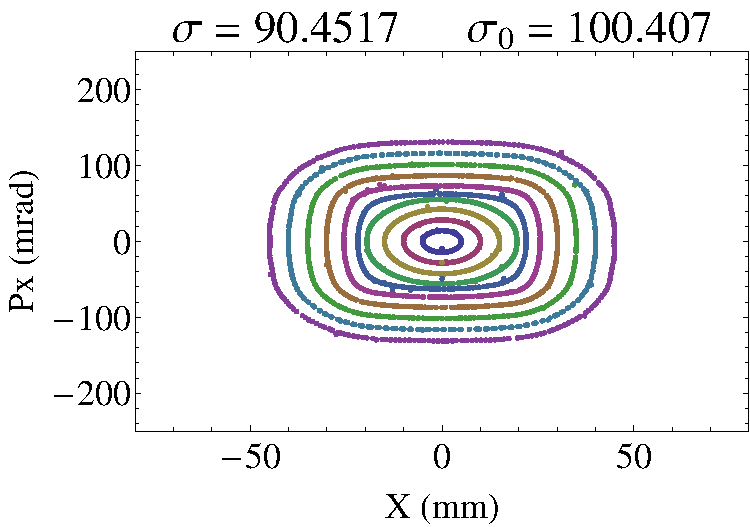
\includegraphics[width=\textwidth]{Img/TestParticle1.pdf}
        \caption{}\label{sfig:TestPtc1}
    \end{subfigure}
    \begin{subfigure}[b]{0.24\textwidth}
        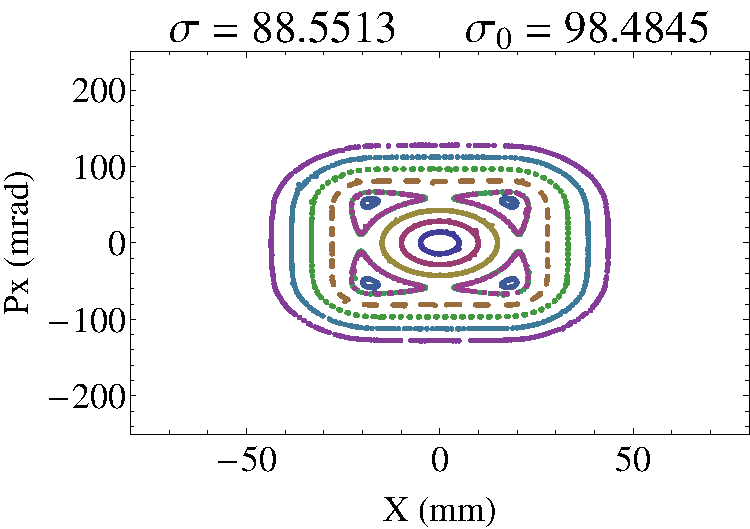
\includegraphics[width=\textwidth]{Img/TestParticle2.pdf}
        \caption{}\label{sfig:TestPtc2}
    \end{subfigure}
    \begin{subfigure}[b]{0.24\textwidth}
        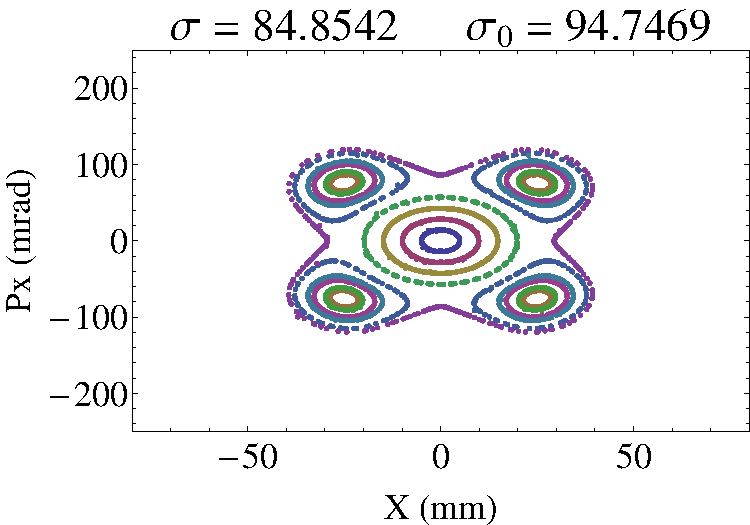
\includegraphics[width=\textwidth]{Img/TestParticle3.pdf}
        \caption{}\label{sfig:TestPtc3}
    \end{subfigure}
    \begin{subfigure}[b]{0.24\textwidth}
        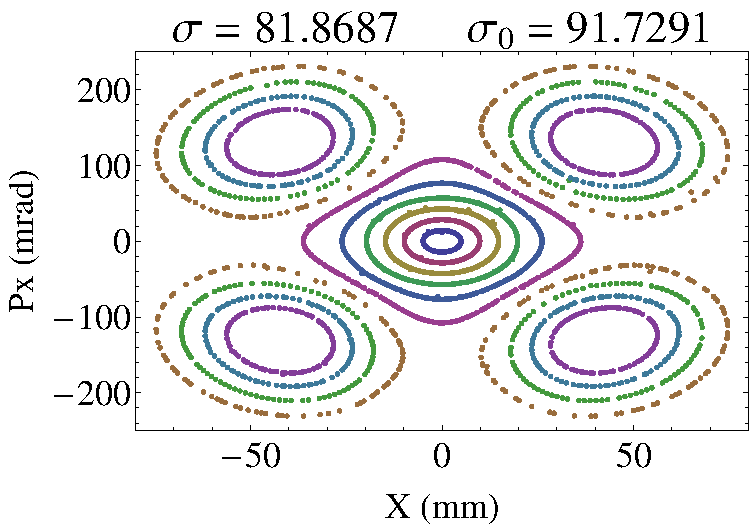
\includegraphics[width=\textwidth]{Img/TestParticle4.pdf}
        \caption{}\label{sfig:TestPtc4}
    \end{subfigure}
    \caption{Poinar\'{e} map from particle core model. Particle-core resonance islands move from inner core to outside in above crossing, Fig.~\ref{sfig:TestPtc1} $\rightarrow$ Fig.~\ref{sfig:TestPtc4}, and conversely in below crossing Fig.~\ref{sfig:TestPtc4}$\rightarrow$Fig.~\ref{sfig:TestPtc1}.}
    \label{fig:TestPtc}
\end{figure}

\begin{figure}[!hbp]
    \centering
    \begin{subfigure}[b]{0.33\textwidth}
        \includegraphics[width=\textwidth]{Img/7595Ptc002050.pdf}
        \caption{}
        \label{sfig:Ptc2tails1}
    \end{subfigure}
    \begin{subfigure}[b]{0.33\textwidth}
        \includegraphics[width=\textwidth]{Img/9575Ptc001800.pdf}
        \caption{}
        \label{sfig:Ptc2tails2}
    \end{subfigure}
    \caption{Phase space profiles around a) period 205 in crossing from below, b) period 180 in crossing from above.}
    \label{fig:Ptc2tail}
\end{figure}


\subsection{总结}
\label{section:Crossing_Summary}
As a follow-up to our previous analytical study of the structure resonance,
this paper studies how the beam is spontaneously affected by the structure
resonances. Since the analytical studies are based on the KV beam distribution
assumption and the linearized perturbation theory, the nonlinear damping effect
and the resonance saturation effect are not included.  The study in this paper
clearly shows the transient behavior of the beam when the structure resonance
stop band is crossed. The mixed 2nd/4th order coherent structure resonance
gives quite reasonable explanation to the results obtained from the PIC
simulations. It must be emphasized again that the interaction between the beam
and the resonances needs to be studied in a transient sense. The ``attractive''
and ``repulsive'' effect of the stop band is a spontaneous beam reaction since
the rms characteristics are modified by the structure resonance. It is also
found that the beam emittance growth is almost linearly proportional to the
time that the beam is affected by the structure resonance. The final beam
equilibrium status is a comprehensive result as a comprise of the structure
resonance and the nonlinear damping. The incoherent particle-core resonance
can cause phase space distortion, emittance growth, and beam halo formation,
but only on a long-time scale.

Another importance is that our simulation clearly proves the conclusion from
our former theoretical prediction, that the lower order stop bands are
naturally included in higher order stop bands.  The study on higher order of
structure resonance can be easily extended and understood in the same frame
discussed here.
One example is the 3rd/6th mixed structure resonance around $60^{\circ}$
phase advance $3 \times 60^{\circ} = 180^{\circ}$,
$6 \times 60^{\circ} = 360^{\circ}$[16] and $120^{\circ}$ phase advance
$3 \times 120^{\circ} = 360^{\circ}$, $6 \times 120^{\circ} = 720^{\circ}$
~\cite{11,36}. The understanding of the coherent and incoherent resonance in
space charge physics leads us to a better understanding of recent experimental
results~\cite{31,32,33}. However, despite the progress in interpretation of the
nonlinear phenomena, there is still a large gap between analytical, numerical
prediction and the experiment. In the near future, further study will be focused
on the extensive study on the real 6D particle dynamics.

\section{小结}                    \label{section:Simulation_conclusion}
通过对并行程序的性能测试可以看出,对于PIC算法在单个普通家用GPU(GTX 1060)上相对于单核CPU实现了超过50倍的加速。
当模拟使用的粒子数较大时,PIC算法在GPU集群上也显示出良好的可扩展性;而当粒子数目较小时其可扩展性较差。

对于Symplectic算法,在一个普通家用GPU上相对于单核CPU实现了接近500倍的加速比。
同时,我们在GPU集群泰坦上的测试还显示出这种算法有良好的可扩展性,程序的加速比随着GPU数目几乎线性增加。

我们在周期性聚焦结构中使用Symplectic算法进行了几个应用模拟,当工作点远离共振线时,束流不会出现发射度增长,而当其接近共振线时发射度会持续增长。
在未来的研究中,我们将继续扩展此模型速发,并在不同架构的计算机上比较保辛算法的效率。

之后,我们使用P-TOPO程序对C-ADS注入器I的RFQ和超导段分别进行了模拟并且与其他程序进行了比较。
模拟结果证明了现有设计的合理性,束团的尺寸和发射度都得到了有效控制,束损以及能散也在合理范围之内,完全满足需求。
之后,我们将继续对P-TOPO进行拓展并加入更多新的功能,以满足强流加速器的各种需求。

最后,我们使用P-TOPO程序对加速器中的共振穿越进行了研究。